\documentclass{article}

\usepackage{graphicx}
\usepackage{float}

\usepackage{polski}
\usepackage[utf8]{inputenc}
\usepackage{indentfirst}

\usepackage{listings}
\usepackage{csvsimple}

\usepackage{pdfpages}
\usepackage{siunitx}

\usepackage{mdframed}
\usepackage{alltt}

\begin{document}

\definecolor{codegreen}{rgb}{0,0.6,0}
\definecolor{codegray}{rgb}{0.5,0.5,0.5}
\definecolor{codepurple}{rgb}{0.58,0,0.82}
\lstdefinestyle{scilab}{
    backgroundcolor=\color{white},
    commentstyle=\color{codegreen},
    keywordstyle=\color{codepurple},
    numberstyle=\tiny\color{black},
    stringstyle=\color{red},
    basicstyle=\footnotesize,
    breakatwhitespace=false,
    breaklines=true,
    keepspaces=true,
    numbers=left,
    showstringspaces=false,
}

\title{Labolatorium Programowanie\\Sprawozdanie z zadania nr 10}
\author{Mikołaj Buchwald\\nr indeksu 385542\\mikolaj.buchwald@gmail.com\\mb83904@st.amu.edu.pl}
\maketitle
% % %

\begin{abstract}
    W ninejeszym sprawozdaniu zamieszczono informacje dotyczące przetwarzania sygnału pochodzącego z elektroencefalografu (EEG). Sygnał, który przetwarzany był na potrzeby tego sprawozdania pochodzi ze 128-elektrodowego EEG.
    
    Rozróżnia się kilka zakresów częstotliwości sygnału EEG. Podział ten oparty jest na podwyższonej amplitudzie pewnych częstotliwości przy wykonywaniu określonych zadań poznawczych (lub stanie odpoczynku bądź snu). Opisano tu pięć rodzajów fal (rytmów): alfa, beta, gamma, delta oraz theta. Dla każdego rodzaju fal wybrano charakterystyczną elektrodę. Surowy sygnał pochodzący z poszczególnych elektrod został przefiltrowany za pomocą filtra środkowoprzepustowego (zakres przepustowości zależny od charakterystyki fal). Przedstawiono po dwa wykresy dla każdej z elektrod: 2-sekundowy przebieg sygnału w dziedzinie czasu oraz  widmo tego 2-sekundowego fragmentu.
    
    Do przetwarzania sygnału oraz wygenerowania wykresów użyto programu Scilab. Skrypt, za pomcą którego wykonano wszystkie operacje załączony jest na końcu tego sprawozdania.
\end{abstract}
% % % % %

%%%%%%%%%%%%%%%%%%%%%%%%%%%%%%%%%%%%%%%%%%%%%%%%%%%%%%%%%%%%%%%%
%        DATA    DATA    DATA    DATA
%%%%%%%%%%%%%%%%%%%%%%%%%%%%%%%%%%%%%%%%%%%%%%%%%%%%%%%%%%%%%%%%
\newpage
\section{Opis zbioru danych}
    Surowy sygnał ze 128-elektrodowego  EEG.  Częstotliwość próbkowania dla sprzętu, z którego pochodzą poniższe dane wynosi 256. Zatem sygnał pobierany był 256 razy na sekundę. Całe badanie trwało prawie 25 sekund. Osoba badana najpierw przez 5 sekund dopoczywała. Następnie przez 15 sekund wykonywała zadanie. Ostatnie niecałe 5 sekund znów było przeznaczone na odpoczynek. 
    Cała tabela ma 128 wierszy oraz 6379 kolumn. Zamieszczono tutaj tylko przykładowe pierwsze 9 wierszy i 3 kolumny.
    \newline
    \begin{table}[h]
        \begin{center}
        \caption[Table caption text]{Sygnał EEG z 128 elektrod zbierany przez 1554 sekundy.}
        \csvautotabular{eeg_128.csv}
        \end{center}
    \end{table}

    Na następnej stronie znajduje się rozkład elektrod w 128-elektrodowym EEG na czaszce człowieka. Numery A1-A32 oznaczono dalej w sprawozdaniu także jako wartości w nawiasach (1-32). Podobnie dla B1-B32 (33-64), C1-C32 (64-96) oraz D1-D32 (97-128). Na grafice oznaczono też elektrody odpowiadające standardowemu rozkładowi elektrod 10-20. 
    \newpage
    \begin{figure}[H]
        \begin{center} 
        \vspace{3cm}
        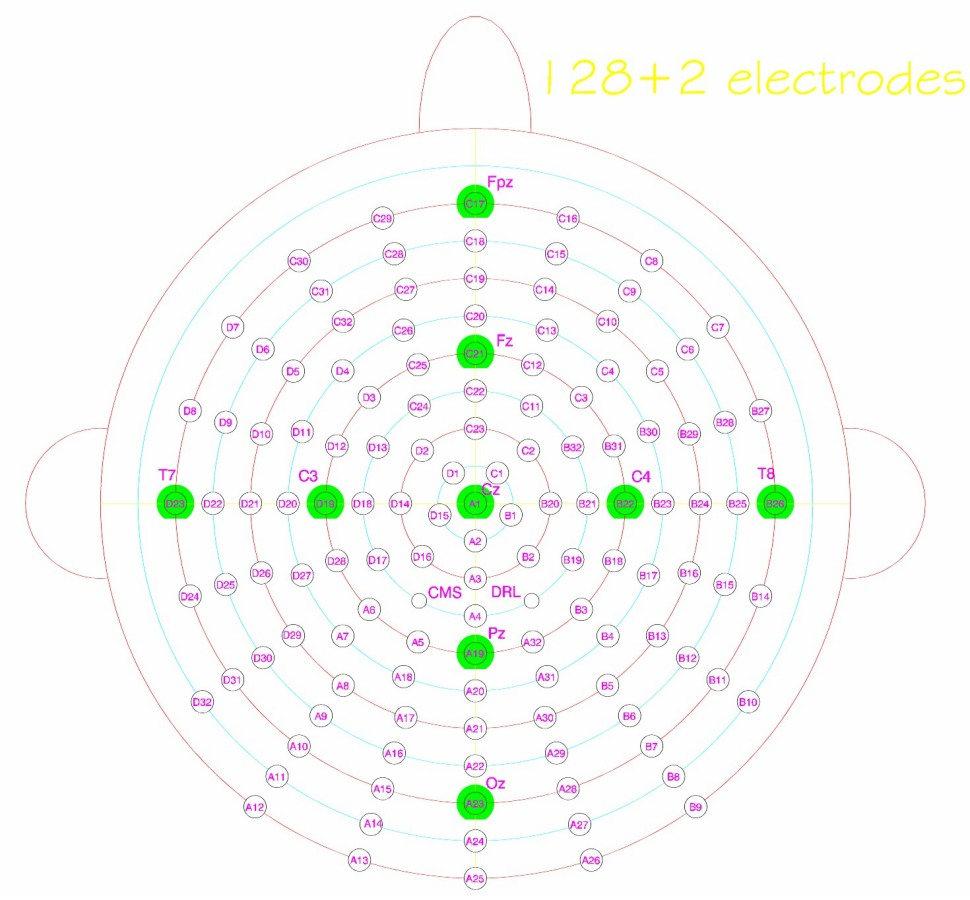
\includegraphics[width=\linewidth]{cap_128_layout_medium.jpg}
        \caption{Rozkład elektrod w 128-elektrodowym EEG}
        \end{center}
    \end{figure}

    \newpage
% % %

%%%%%%%%%%%%%%%%%%%%%%%%%%%%%%%%%%%%%%%%%%%%%%%%%%%%%%%%%%%%%%%%
%        ALPHA    ALPHA    ALPHA    ALPHA
%%%%%%%%%%%%%%%%%%%%%%%%%%%%%%%%%%%%%%%%%%%%%%%%%%%%%%%%%%%%%%%%
\newpage
\section{Fale alfa ($\alpha$)}
    %

    \subsection{Czym są i gdzie występują fale alfa}
    
    Częstotliwość charakterystyczna dla fal alfa to 8-13 Hz. Amplituda fal waha się od 20-100 \si{\micro\volt}.\\

    Fale alfa obserwuje się gdy osoba badana jest w stanie spoczynku i ma zamknięte oczy, zarazem zachowując świadomość. Tyczy się to głównie osób dorosłych. W przypadku zajścia procesów uwagowych bądź wystąpienia bodźców zewnętrznych stwierdza się zanik wspomnianych fal.\\

    Występowanie fal o tym zakresie można zarejestrować w okolicach potylicznych, ciemieniowo-potylicznych oraz skroniowo-potylicznych.\\

    Na potrzeby tego zadania wybrana została elektroda A21 (21). Znajduje się ona w części potylicznej, potyliczno-ciemieniowej czaszki. Poniżej zaprezentowano 2-sekundowy przebieg w dziedzinie czasu dla fal alfa dla tejże elektordy. Przedstawiono też na wykresie widmo tego 2-sekundowego fragmentu dla wspomnianej elektordy A21. Dane te dotyczą 8-10 sekundy badania.
    % %
    \newpage
    \subsection{Fale alfa dla elektrody A21 (21)}
    \begin{figure}[H]
        \hspace*{-1.5cm} 
        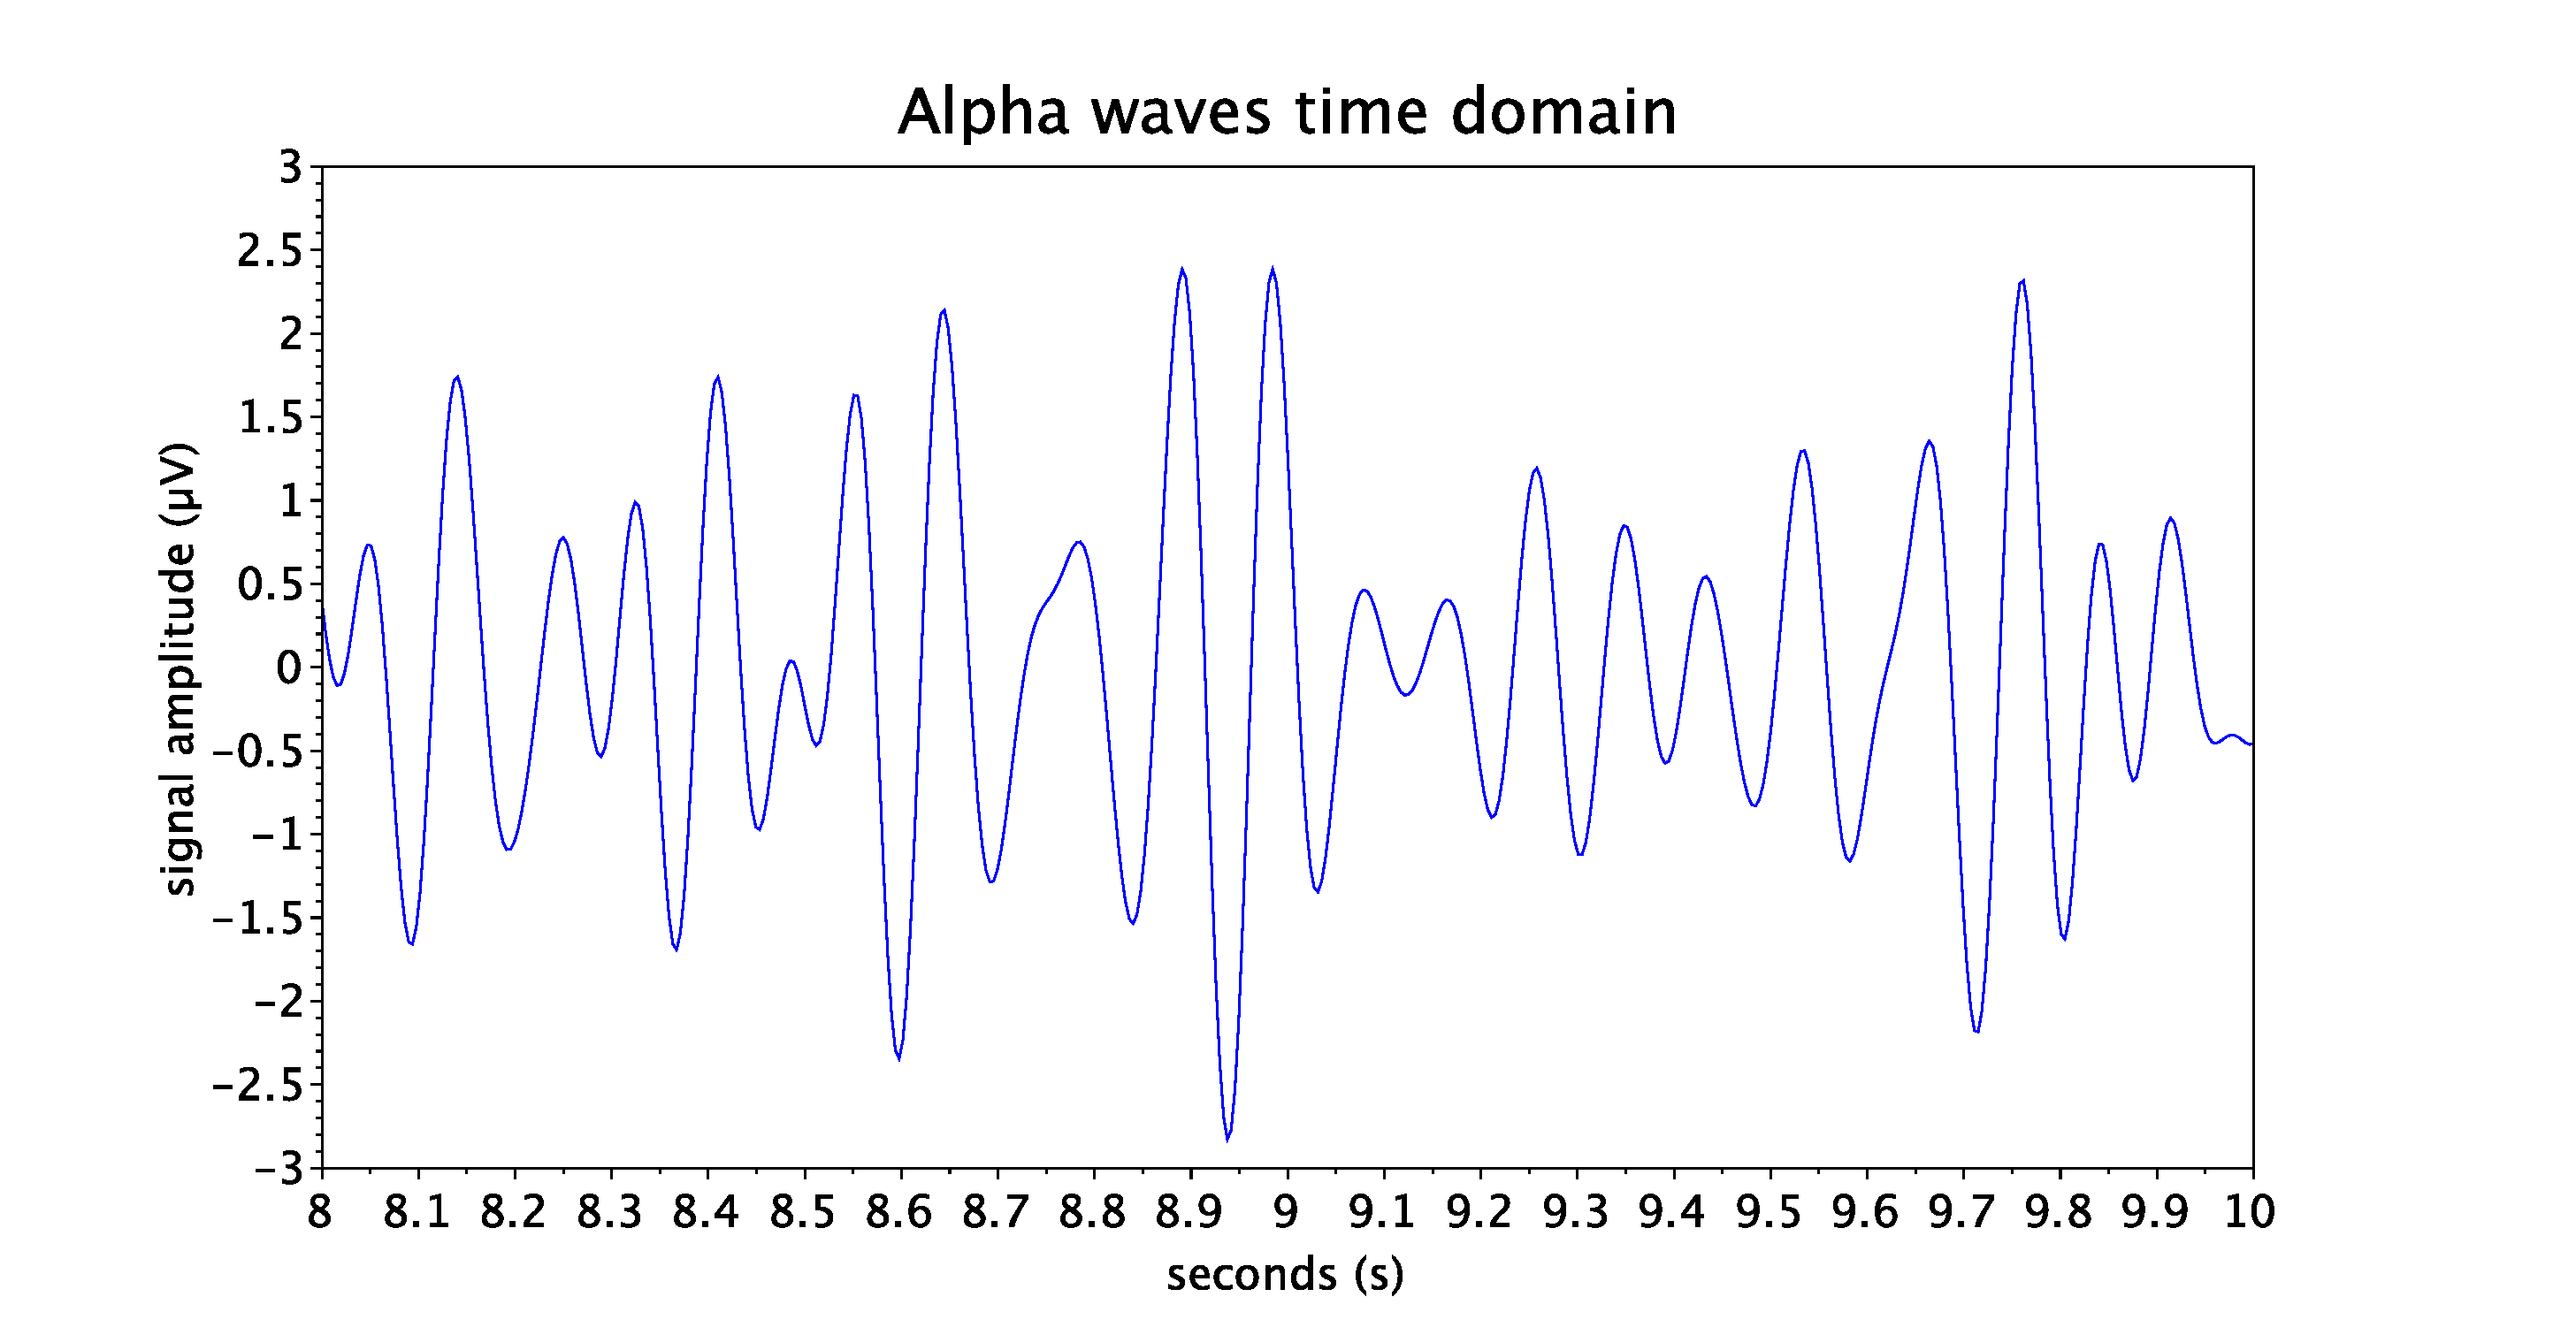
\includegraphics[width=\linewidth+3cm]{alpha_time.pdf}
        \caption{Odczyt EEG z elektrody A21 w dziedzinie czasu}
    \end{figure}
    \begin{figure}[H]
        \hspace*{-1.5cm}
        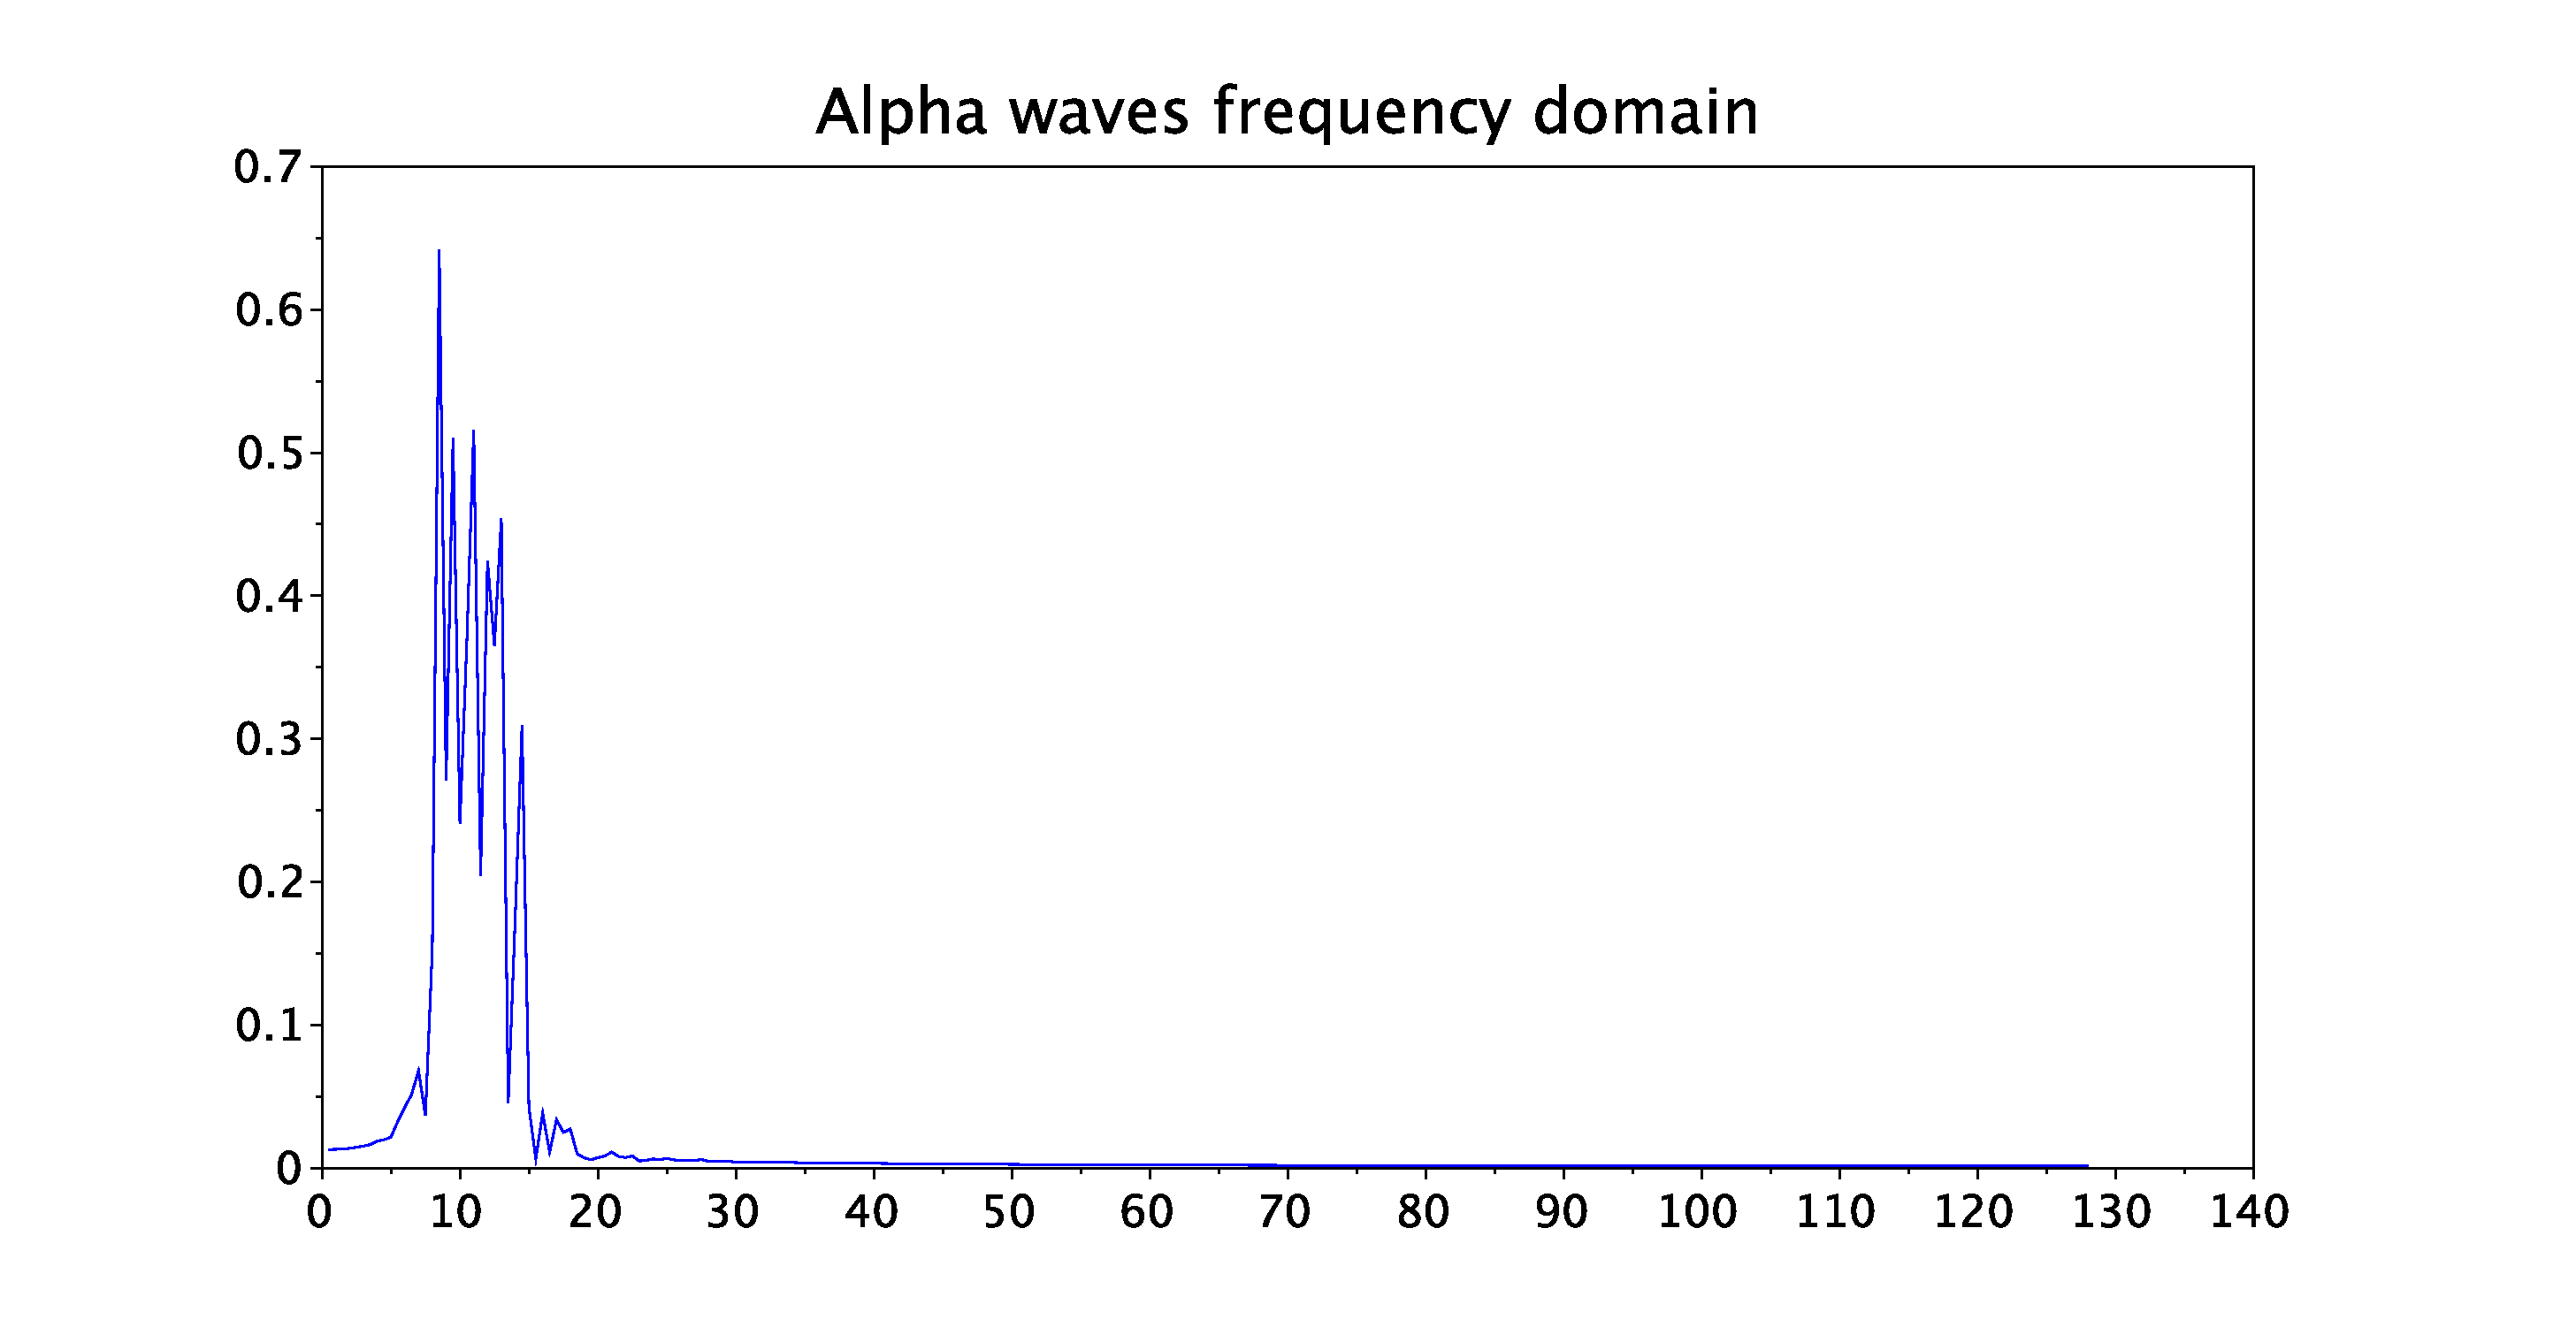
\includegraphics[width=\linewidth+3cm]{alpha_freq.pdf}
        \caption{Odczyt EEG z ele ktrody A21 w dziedzinie częstotliwości}
    \end{figure}
 % % %

%%%%%%%%%%%%%%%%%%%%%%%%%%%%%%%%%%%%%%%%%%%%%%%%%%%%%%%%%%%%%%%%
%        BETA    BETA    BETA    BETA
%%%%%%%%%%%%%%%%%%%%%%%%%%%%%%%%%%%%%%%%%%%%%%%%%%%%%%%%%%%%%%%%
\newpage
\section{Fale beta ($\beta$)}
    %

    \subsection{Czym są i gdzie występują fale beta}
    
    Częstotliwość charakterystyczna dla fal beta to 13-30 Hz. Amplituda fal jest niewielka: do 20 \si{\micro\volt}.\\

    Fale beta obserwuje się gdy osoba badana jest w stanie relaksu i sobie ten stan uświadamia. Fale beta przestaje się rejestrować gdy osoba badana wykona jakiś ruch (zwłaszcza ruch ręki).\\

    Występowanie fal o tym zakresie można zauważyć w przednich częściach mózgu, w okolicach czołowych.\\

    Na potrzeby tego zadania wybrana została elektroda C21 (85). Znajduje się ona w części czołowej czaszki. Poniżej zaprezentowano 2-sekundowy przebieg w dziedzinie czasu dla fal alfa dla tejże elektordy. Przedstawiono też na wykresie widmo tego 2-sekundowego fragmentu dla wspomnianej elektordy C21. Dane te dotyczą 8-10 sekundy badania.
    % %

    \newpage
    \subsection{Fale beta dla elektrody C21 (85)}
    \begin{figure}[H]
        \hspace*{-1.5cm}
        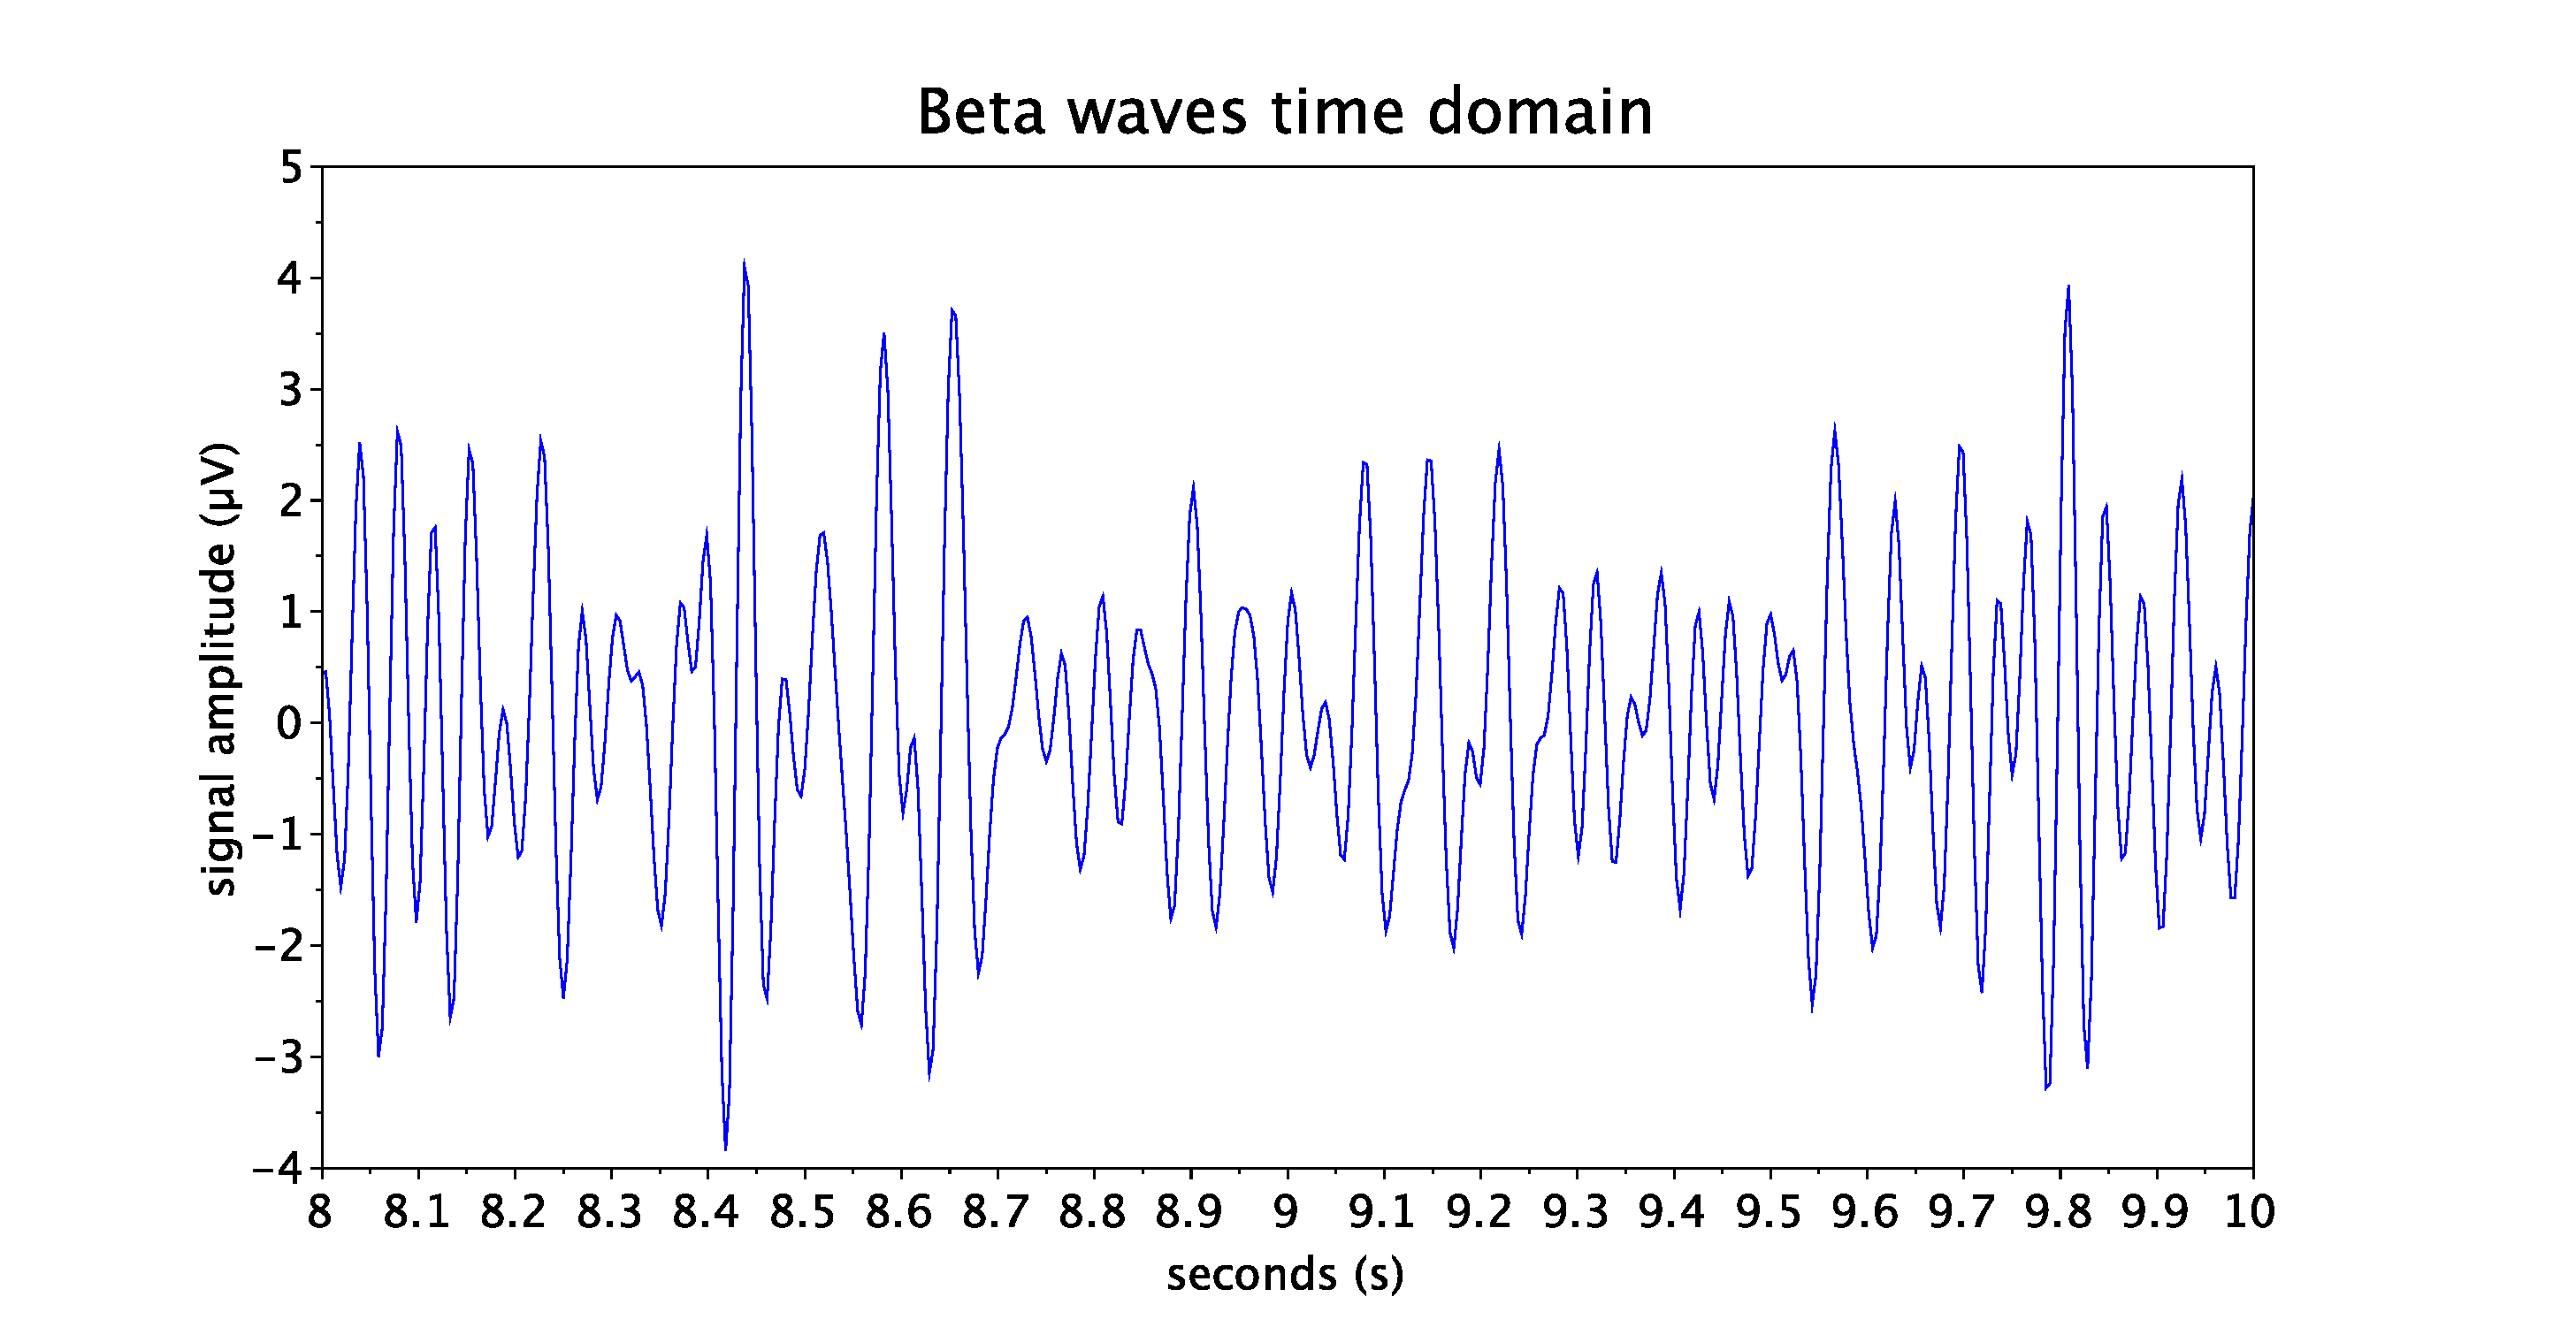
\includegraphics[width=\linewidth+3cm]{beta_time.pdf}
        \caption{Odczyt EEG z elektrody C21 w dziedzinie czasu}
    \end{figure}
    \begin{figure}[H]
        \hspace*{-1.5cm}
        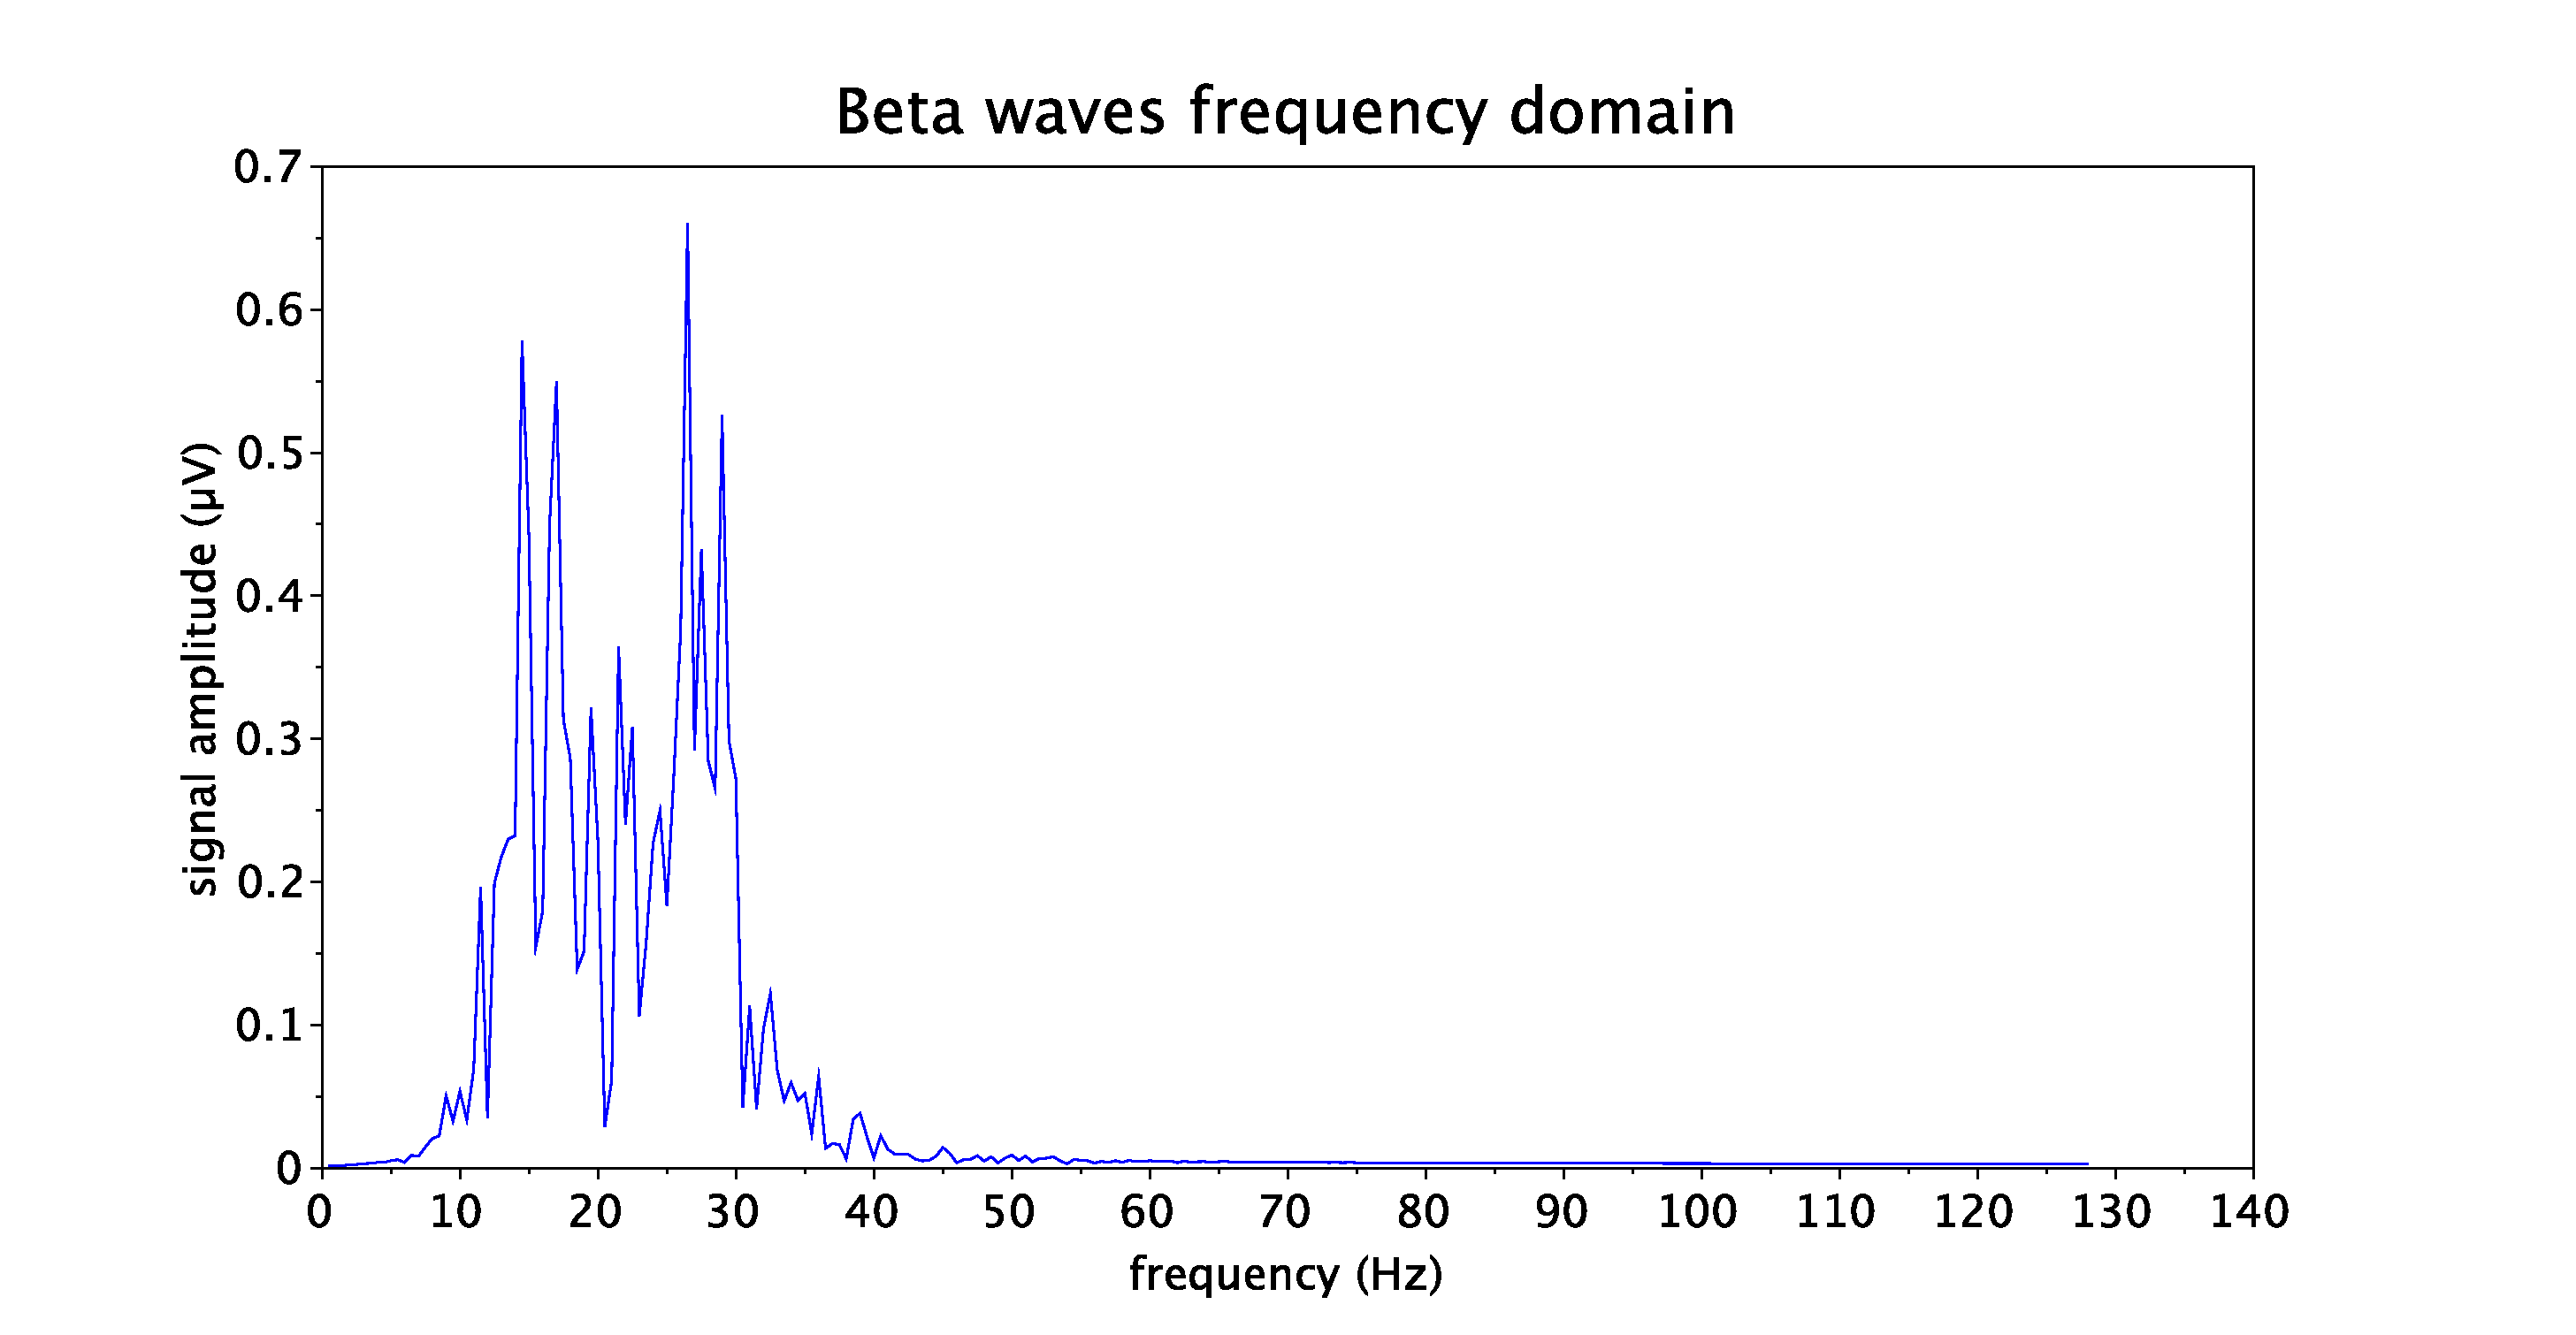
\includegraphics[width=\linewidth+3cm]{beta_freq.pdf}
        \caption{Odczyt EEG z elektrody C21 w dziedzinie częstotliwości}
    \end{figure}
% % %

%%%%%%%%%%%%%%%%%%%%%%%%%%%%%%%%%%%%%%%%%%%%%%%%%%%%%%%%%%%%%%%%
%        GAMMA    GAMMA    GAMMA    GAMMA
%%%%%%%%%%%%%%%%%%%%%%%%%%%%%%%%%%%%%%%%%%%%%%%%%%%%%%%%%%%%%%%%
\newpage
    \section{Fale gamma ($\gamma$)}
    %

    \subsection{Czym są i gdzie występują fale gamma}
    
    Częstotliwość charakterystyczna dla fal gamma to 30-80 Hz. Częstotliwości powyżej 80 Hz określa się mianem fal gamma wysokoczęstotliwościowych. \\

    Fale beta obserwuje się podczas aktywności fizycznej osoby badanej oraz przy aktywowaniu się funkcji motorycznych. Z falami gamma mamy także do czynienia gdy badamy wyższe funkcje poznawcze, percepcję sensoryczną oraz procesy pamięciowe. Wysokie częstotliwości gamma obserwuje się gdy badany poddawany jest bodźcowaniu: tak zewnętrznemu (percepcja zmysłowa) jak i wewnętrznemu (funkcje przygotowania ruchu czy artykulacji).\\

    Występowanie fal o tym zakresie można zauważyć w okolicach kory morotycznej. Jak też i somatosensorycznej.\\

    Na potrzeby tego zadania wybrana została elektroda A3 (3). Znajduje się ona w części czołowo-potylicznej czaszki. Poniżej zaprezentowano 2-sekundowy przebieg w dziedzinie czasu dla fal alfa dla tejże elektordy. Przedstawiono też na wykresie widmo tego 2-sekundowego fragmentu dla wspomnianej elektordy A3. Dane te dotyczą 8-10 sekundy badania.
    % %
    
    \newpage
    \subsection{Fale gamma dla elektrody A3 (3)}
    \begin{figure}[H]
        \hspace*{-1.5cm}
        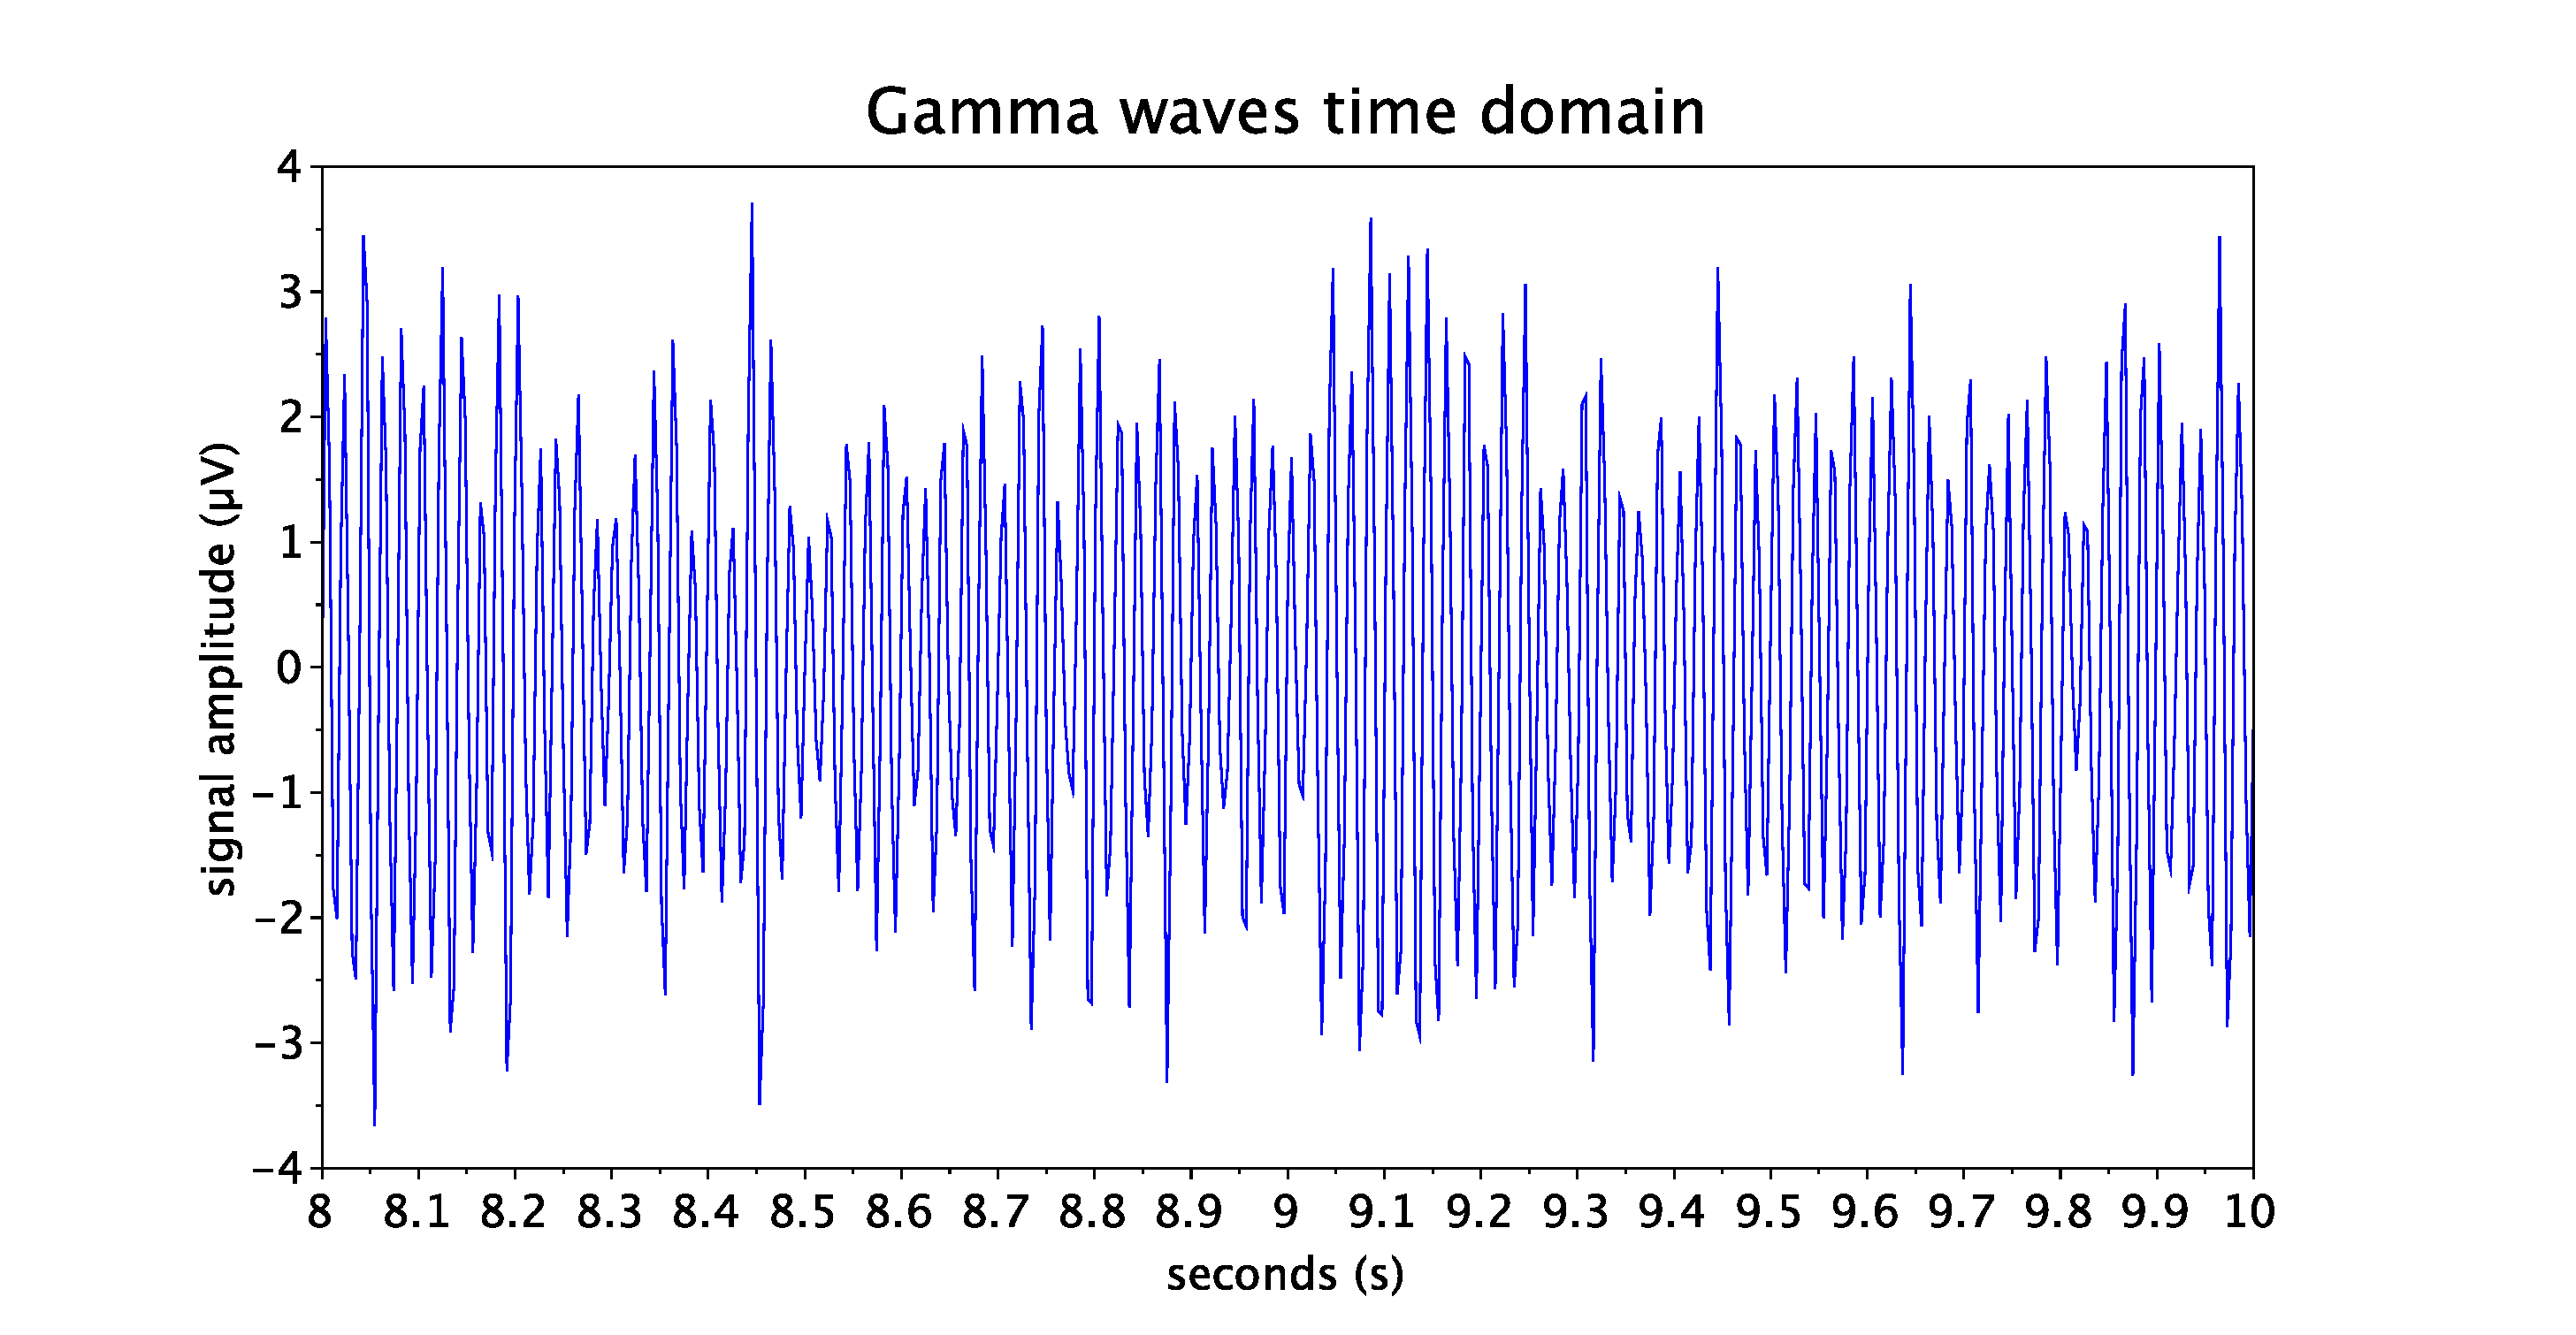
\includegraphics[width=\linewidth+3.2cm]{gamma_time.pdf}
        \caption{Odczyt EEG z elektrody A3 w dziedzinie czasu}
    \end{figure}
    \begin{figure}[H]
        \hspace*{-1.5cm}
        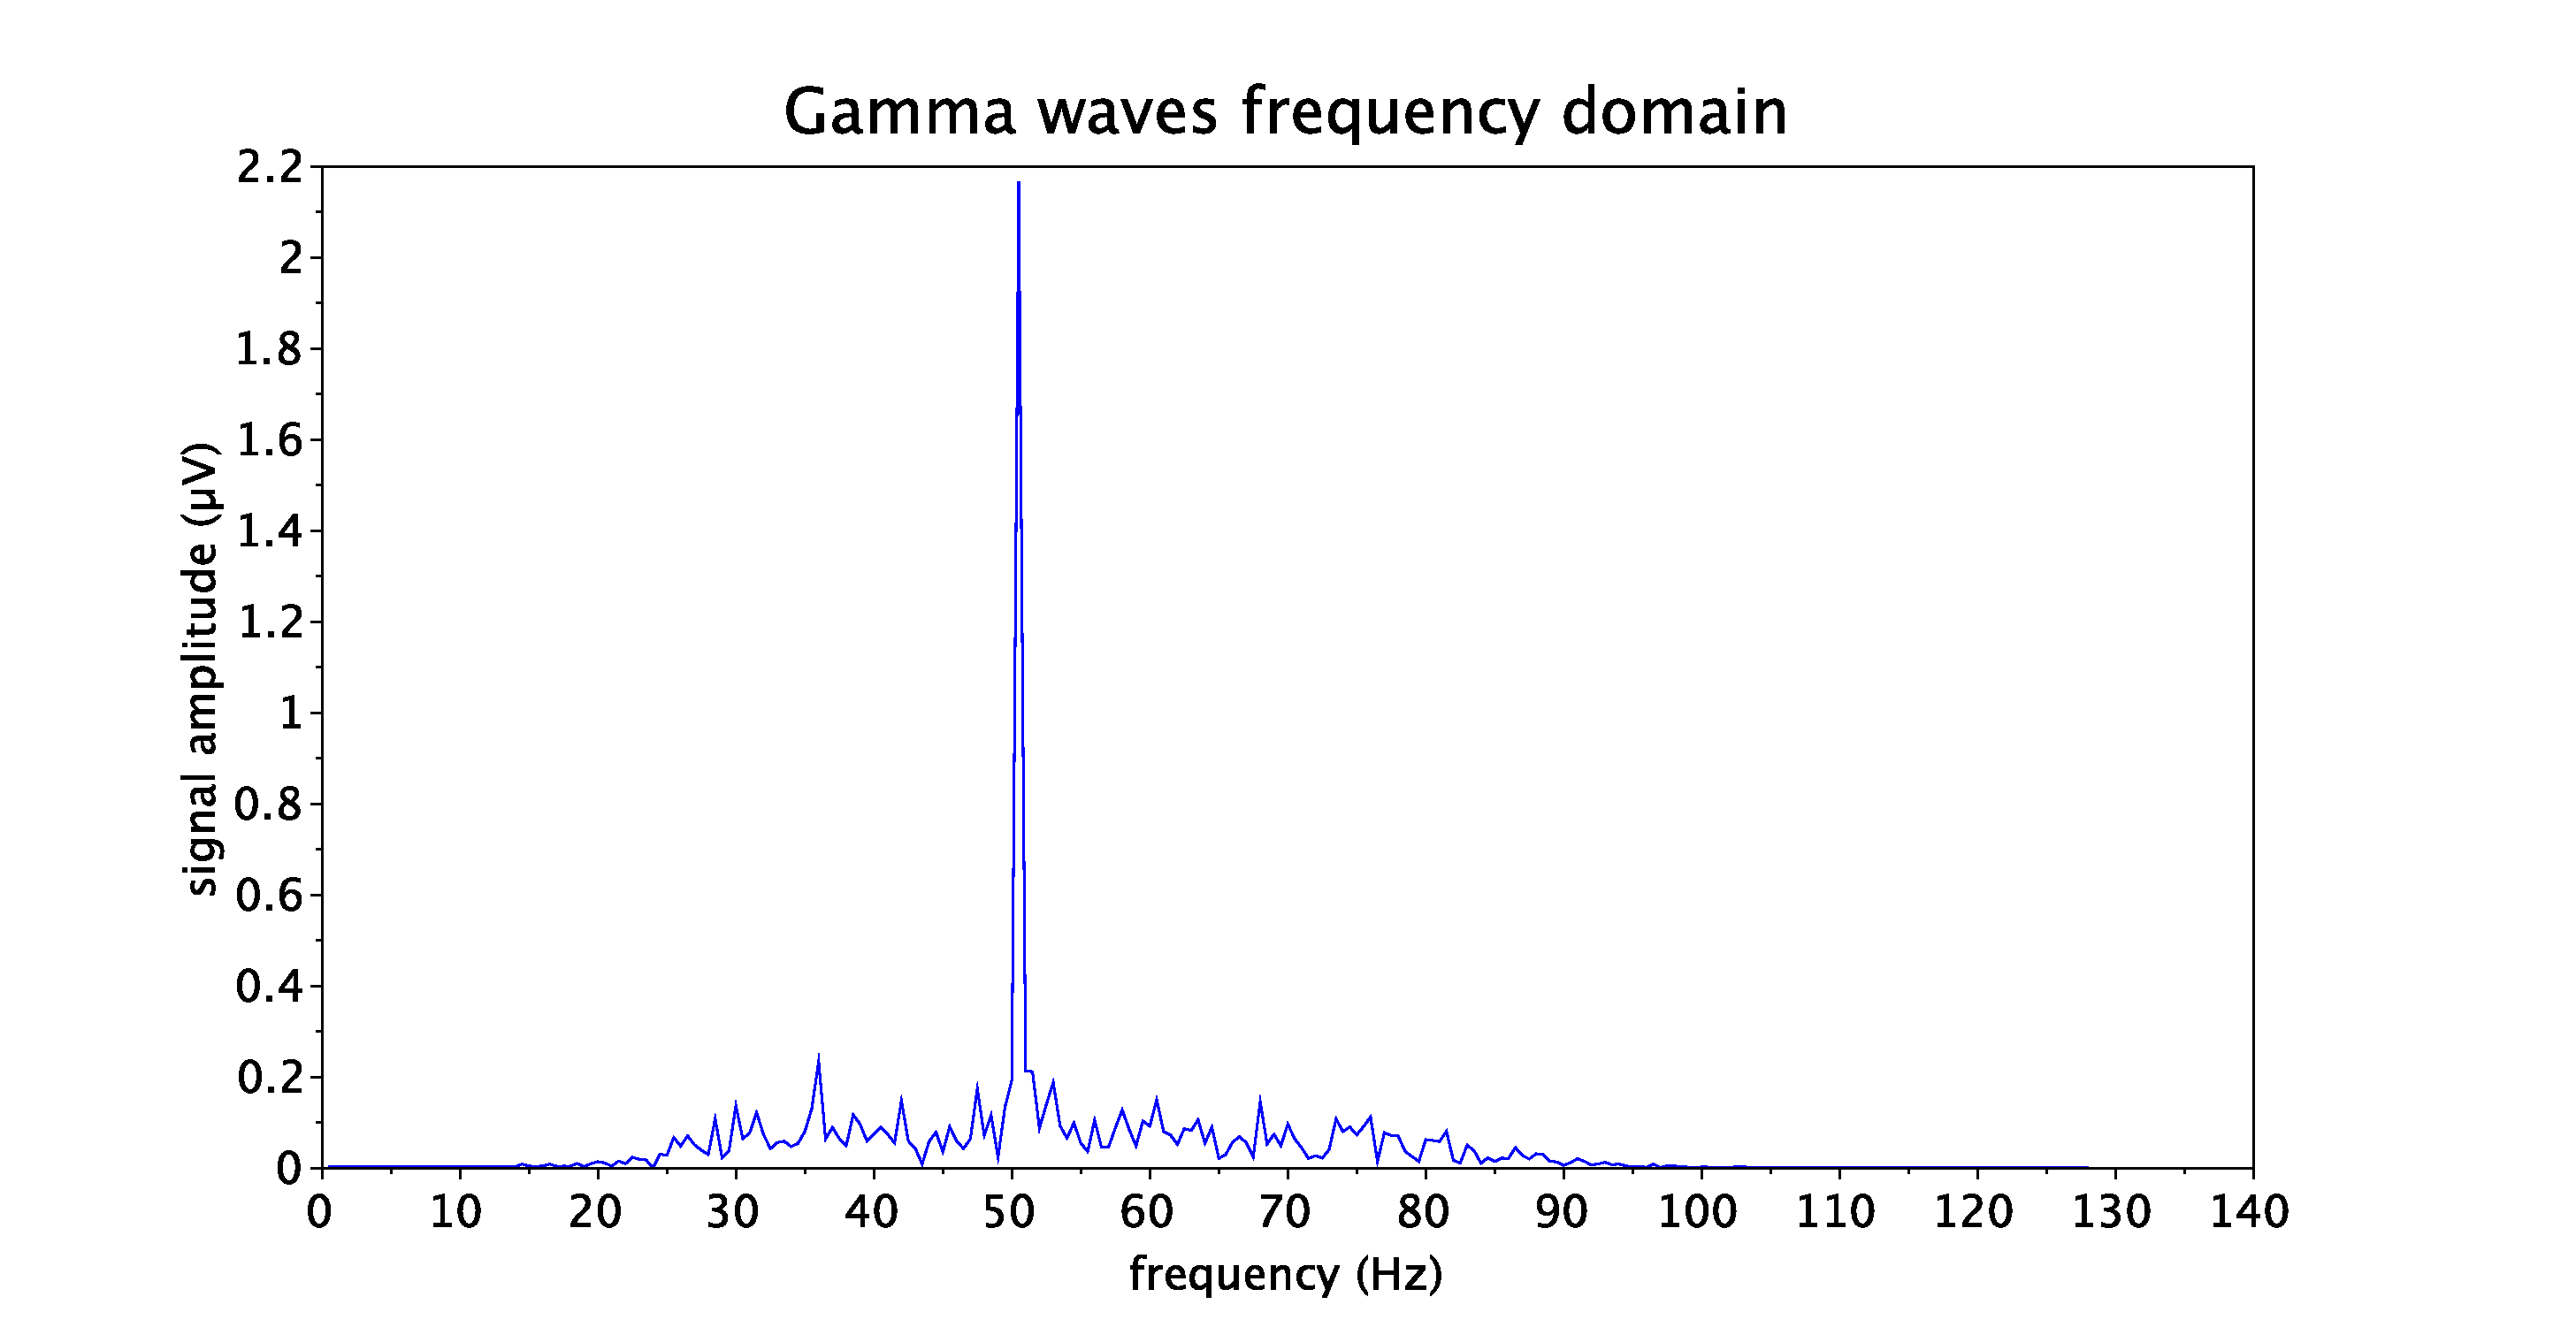
\includegraphics[width=\linewidth+3cm]{gamma_freq.pdf}
        \caption{Odczyt EEG z elektrody A3 w dziedzinie częstotliwości}
    \end{figure}
% % %

%%%%%%%%%%%%%%%%%%%%%%%%%%%%%%%%%%%%%%%%%%%%%%%%%%%%%%%%%%%%%%%%
%        DELTA    DELTA    DELTA    DELTA
%%%%%%%%%%%%%%%%%%%%%%%%%%%%%%%%%%%%%%%%%%%%%%%%%%%%%%%%%%%%%%%%
\newpage
\section{Fale delta ($\delta$)}
    %

    \subsection{Czym są i gdzie występują fale delta}

    Charakterystyczne częstotliwości dla fal delta to częstotliwości poniżej 4 Hz. Amplituda tychże fal wynosi 50 \si{\micro\volt}.\\

    Fale delta występują podczas snu. W trzeciej i czwartej fazie snu obserwuje się wzrost amplitudy powyżej 75 \si{\micro\volt}. Poza stanem uśpienia u dzieci oraz w fazach głębokiej medytacji również da się zarejestrować fale delta.\\

    Z przyczyn technicznych do tego zadania założono zakres częstotliwości dla fal delta od 1 do 4 Hz.\\

    Na potrzeby tego zadania wybrana została elektroda C19 (83). Znajduje się ona w części czołowej czaszki. Poniżej zaprezentowano 2-sekundowy przebieg w dziedzinie czasu dla fal alfa dla tejże elektordy. Przedstawiono też na wykresie widmo tego 2-sekundowego fragmentu dla wspomnianej elektordy C19. Dane te dotyczą 8-10 sekundy badania.
    % %

    \newpage
    \subsection{Fale delta dla elektrody C19 (83)}
    \begin{figure}[H]
        \hspace*{-1.5cm} 
        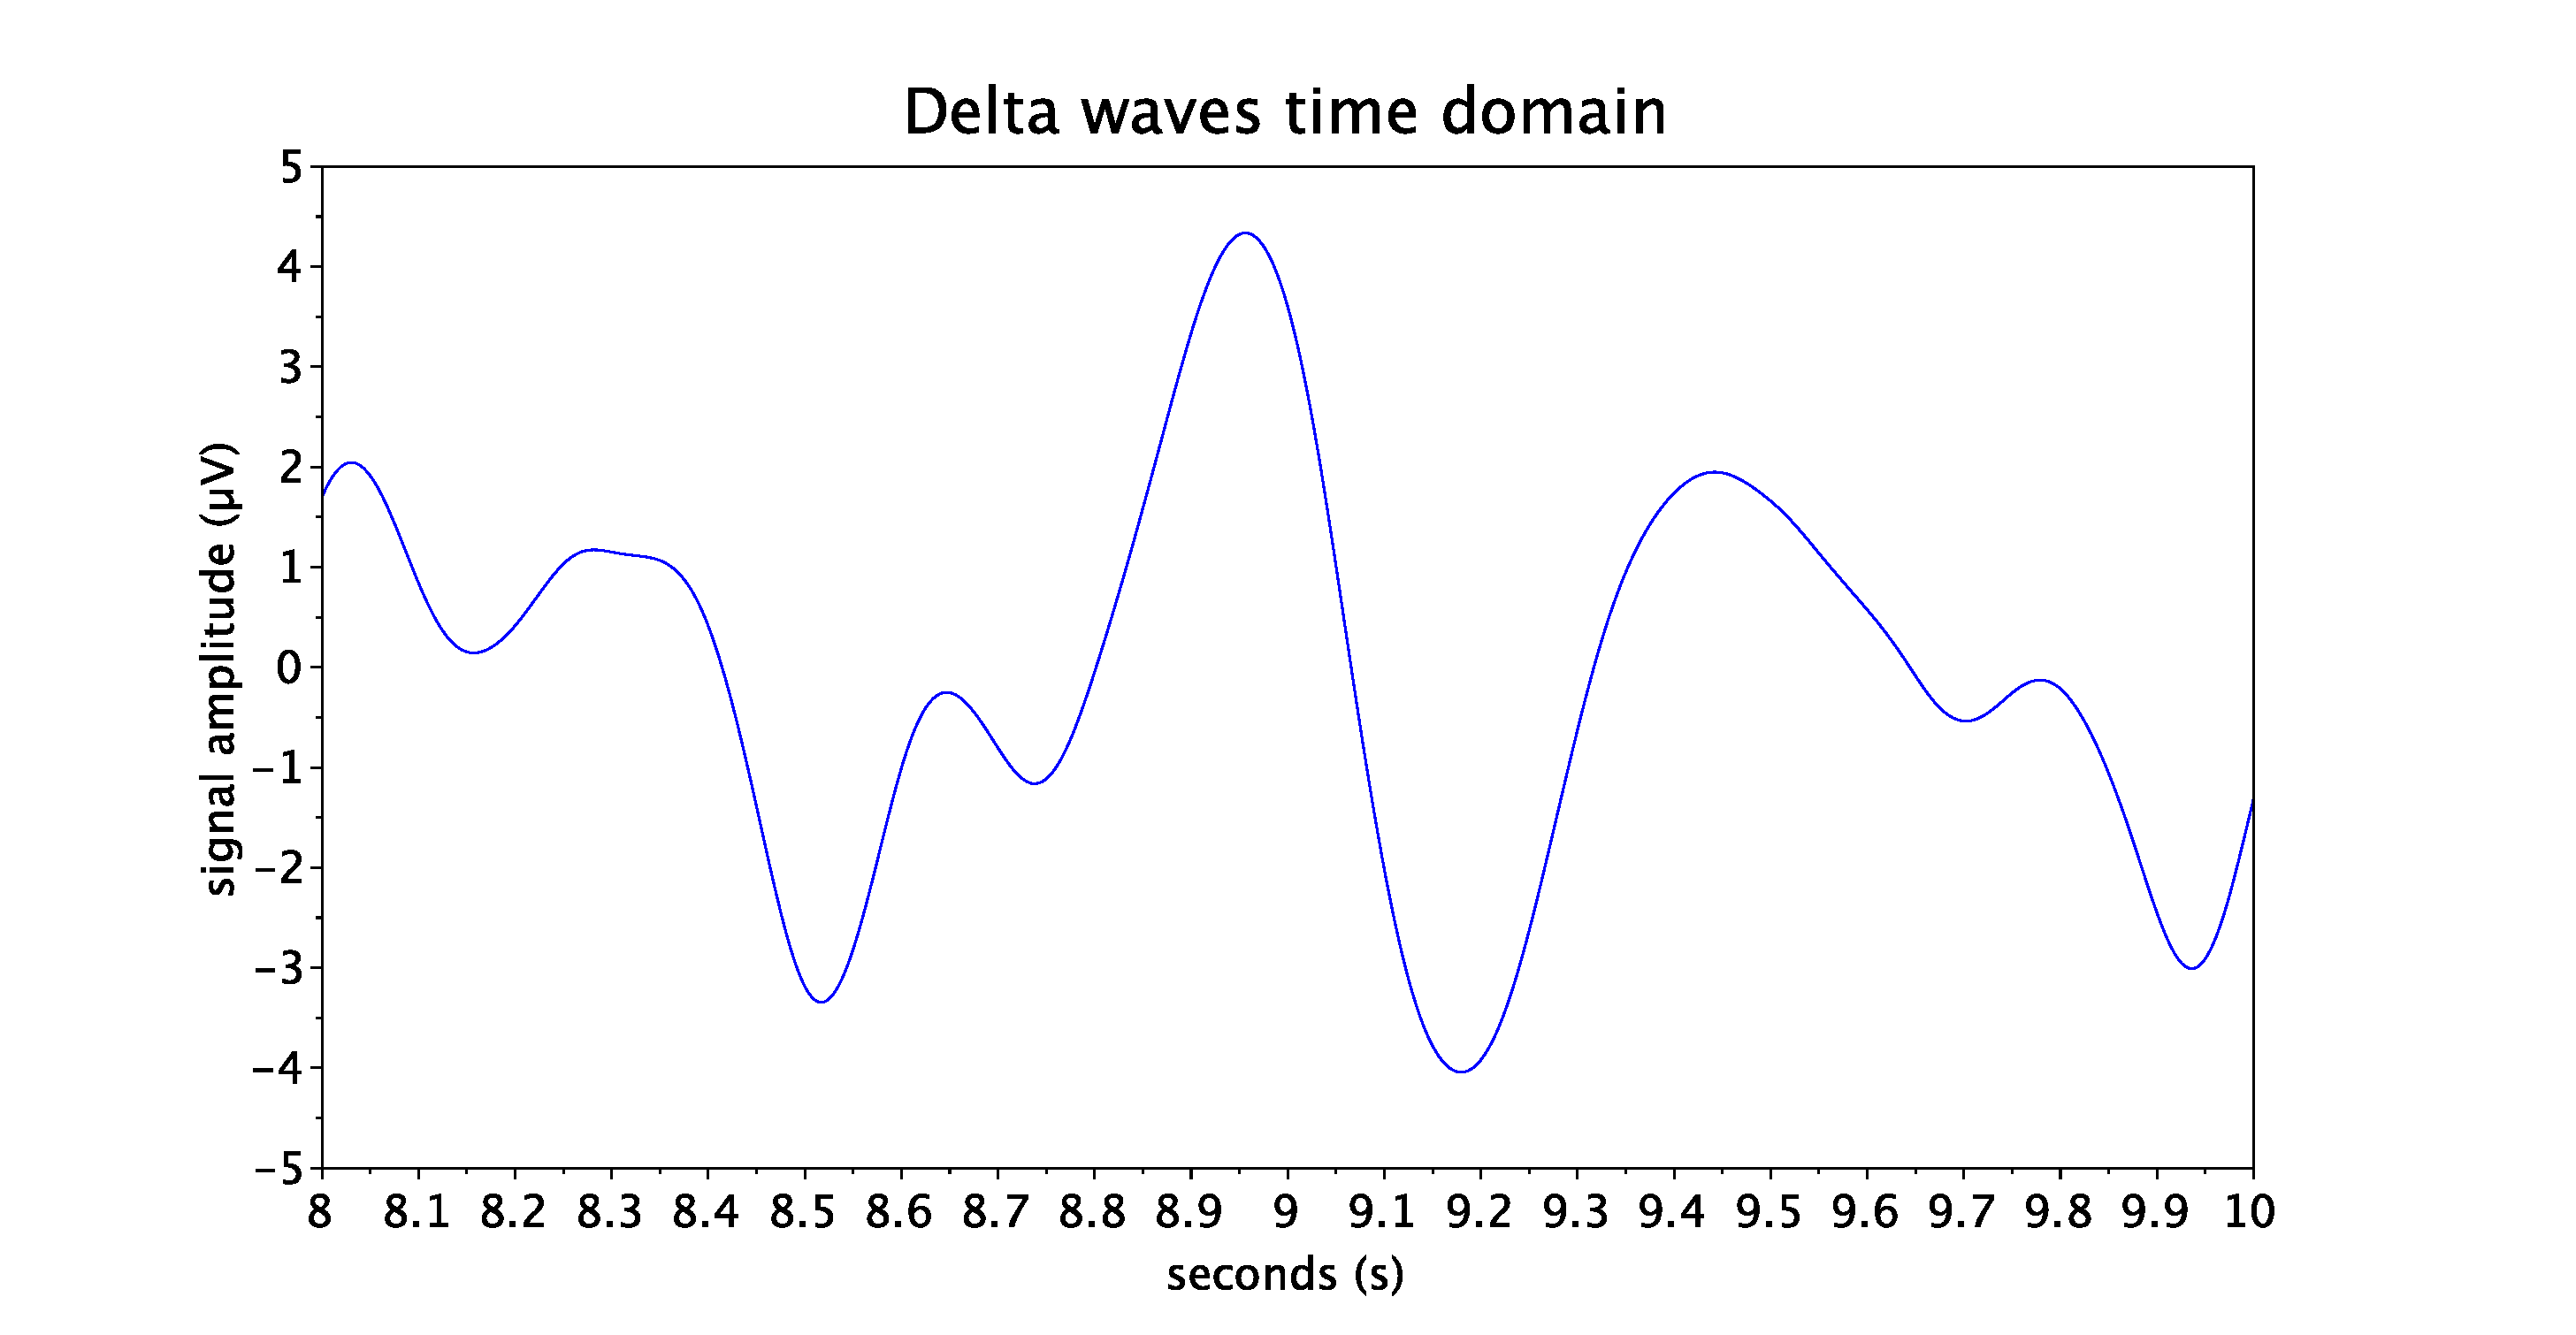
\includegraphics[width=\linewidth+3cm]{delta_time.pdf}
        \caption{Odczyt EEG z elektrody C19 w dziedzinie czasu}
    \end{figure}
    \begin{figure}[H]
        \hspace*{-1.5cm}
        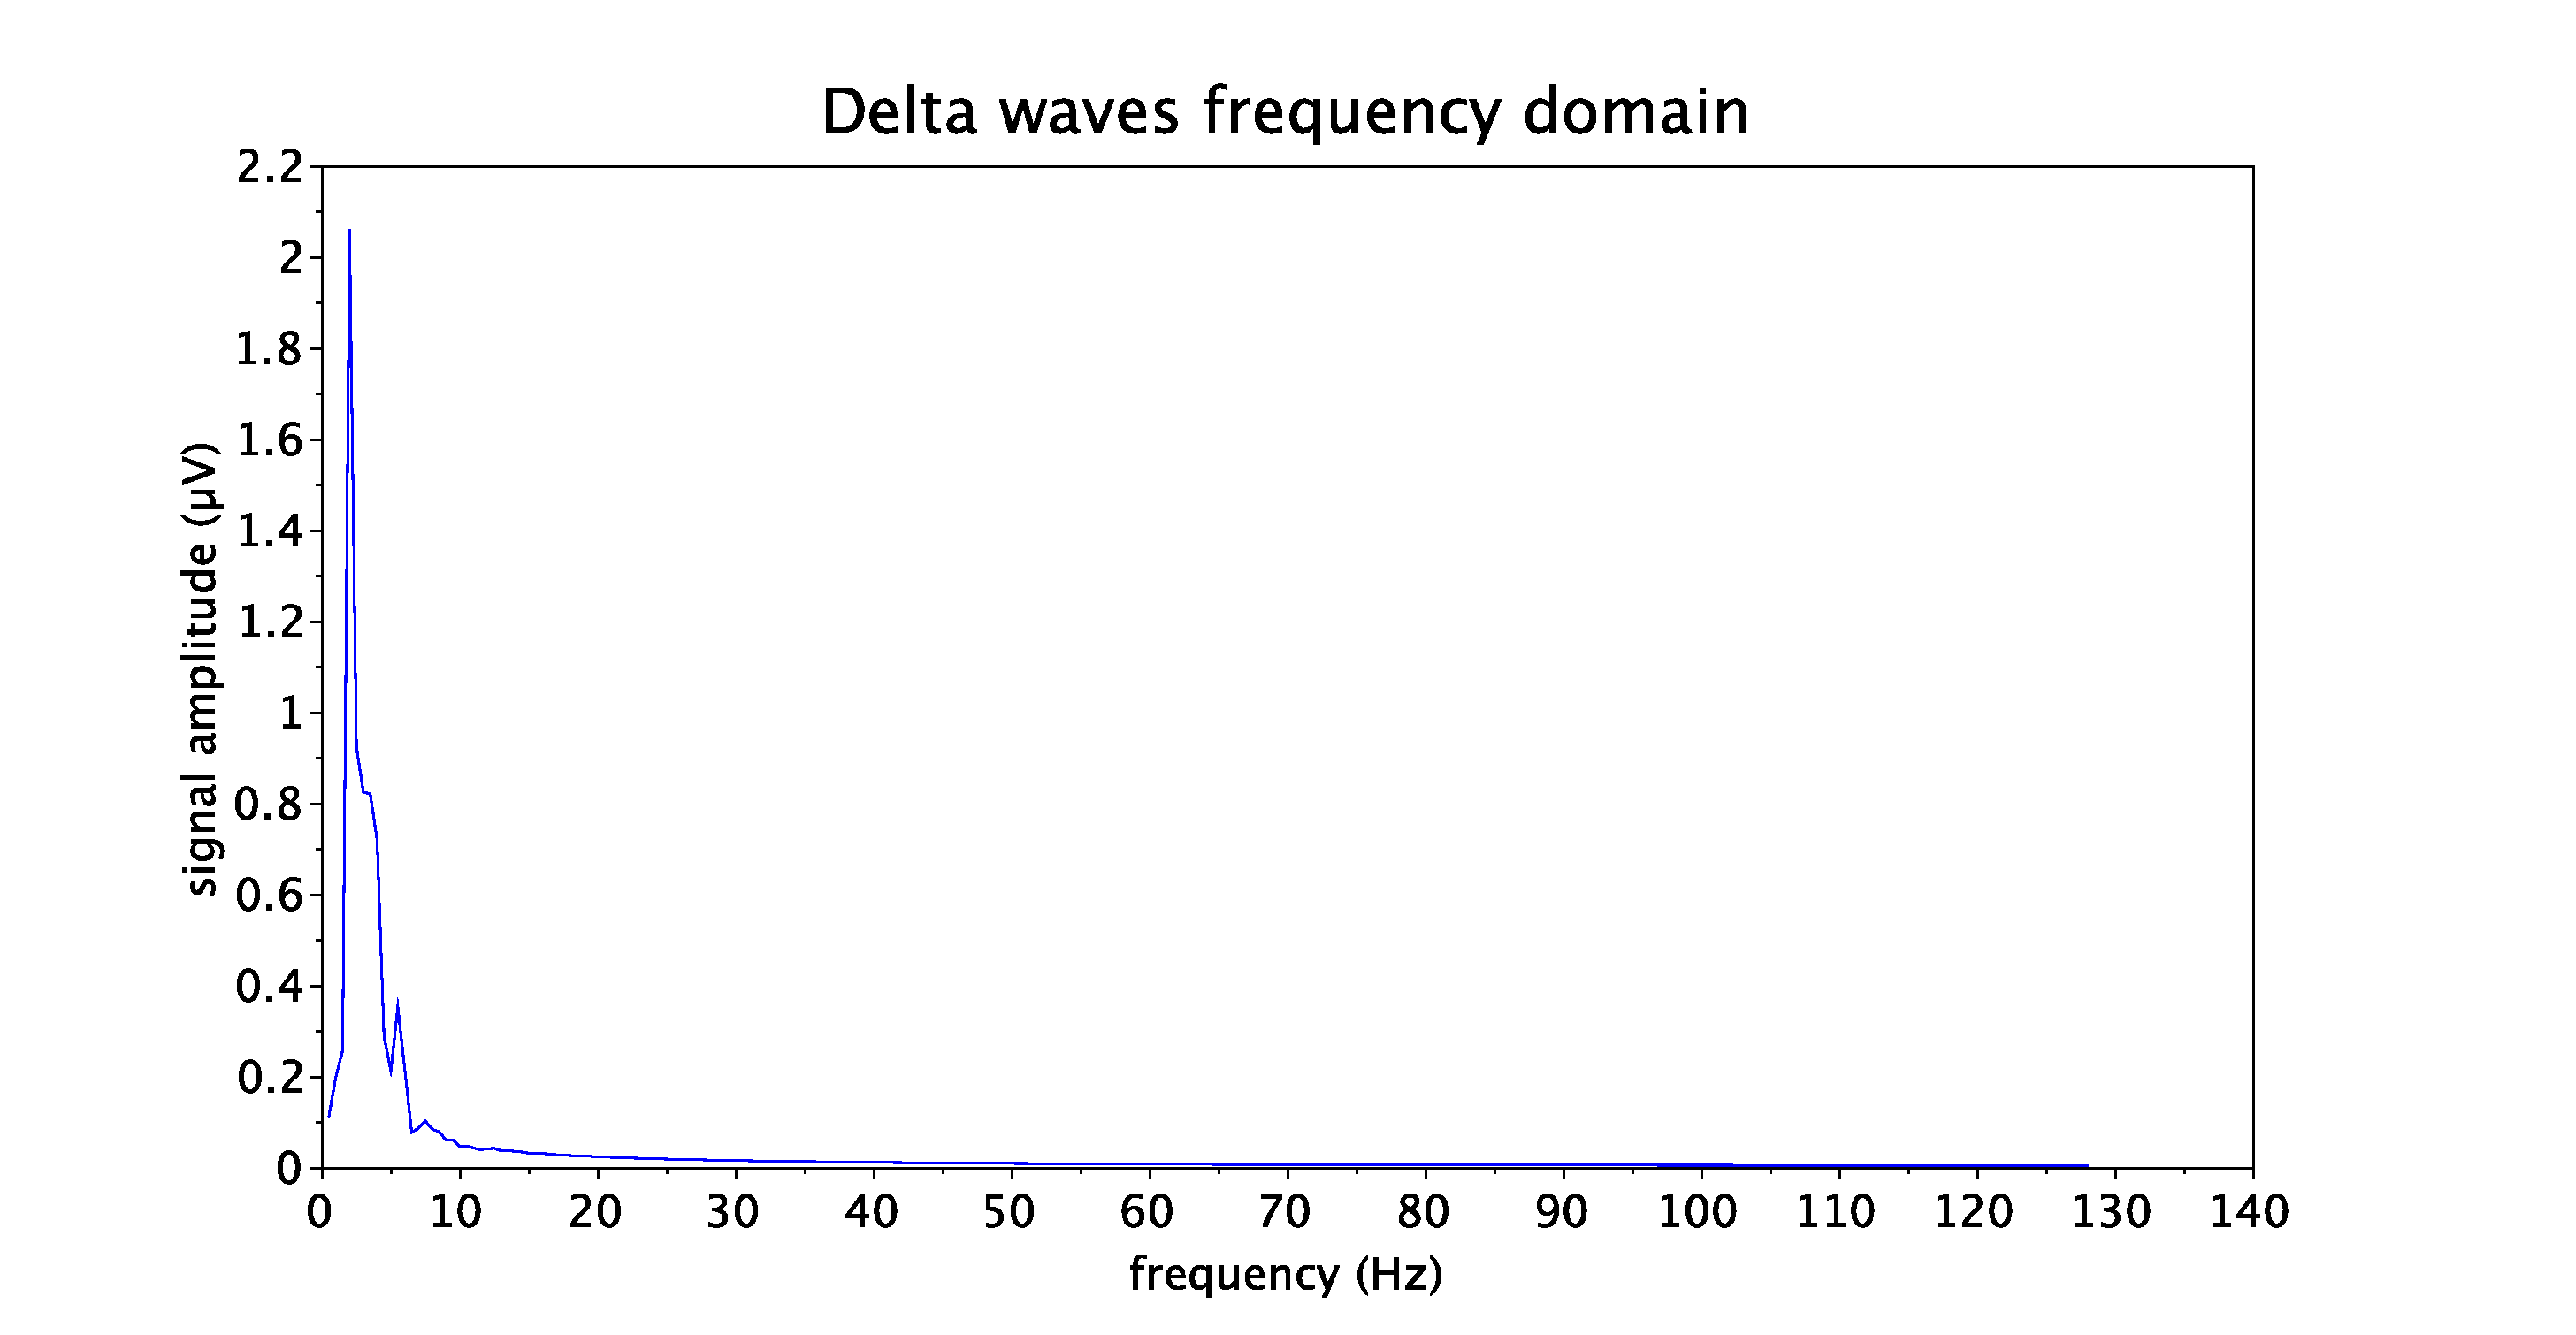
\includegraphics[width=\linewidth+3cm]{delta_freq.pdf}
        \caption{Odczyt EEG z elektrody C19 w dziedzinie częstotliwości}
    \end{figure}
% % %

%%%%%%%%%%%%%%%%%%%%%%%%%%%%%%%%%%%%%%%%%%%%%%%%%%%%%%%%%%%%%%%%
%        THETA    THETA    THETA    THETA
%%%%%%%%%%%%%%%%%%%%%%%%%%%%%%%%%%%%%%%%%%%%%%%%%%%%%%%%%%%%%%%%
\newpage
\section{Fale theta ($\theta$)}
    % 

    \subsection{Czym są i gdzie występują fale theta}

    Zakres częstotliwości dla fal theta to 4-7 Hz. Amplituda fal w tym zakresie to 30 \si{\micro\volt}. Obserwuje się je głównie u dzieci. Fale theta zanikają w okresie dojrzewania. Fale o tej częstotliwości można też wywołać u osób dorosłych za pomocą hiperwentylacji. Również w czasie płytkiego snu czy drzemki rytm theta daje się zarejestrować.\\

    Fale theta występują w przyśrodkowej przedniej części mózgu.\\

    Na potrzeby tego zadania wybrana została elektroda D19 (115). Znajduje się ona w części czołowej czaszki. Poniżej zaprezentowano 2-sekundowy przebieg w dziedzinie czasu dla fal alfa dla tejże elektordy. Przedstawiono też na wykresie widmo tego 2-sekundowego fragmentu dla wspomnianej elektordy D19. Dane te dotyczą 8-10 sekundy badania.
    % %

    \newpage
    \subsection{Fale theta dla elektrody D19 (115)}
    \begin{figure}[H]
        \hspace*{-1.5cm} 
        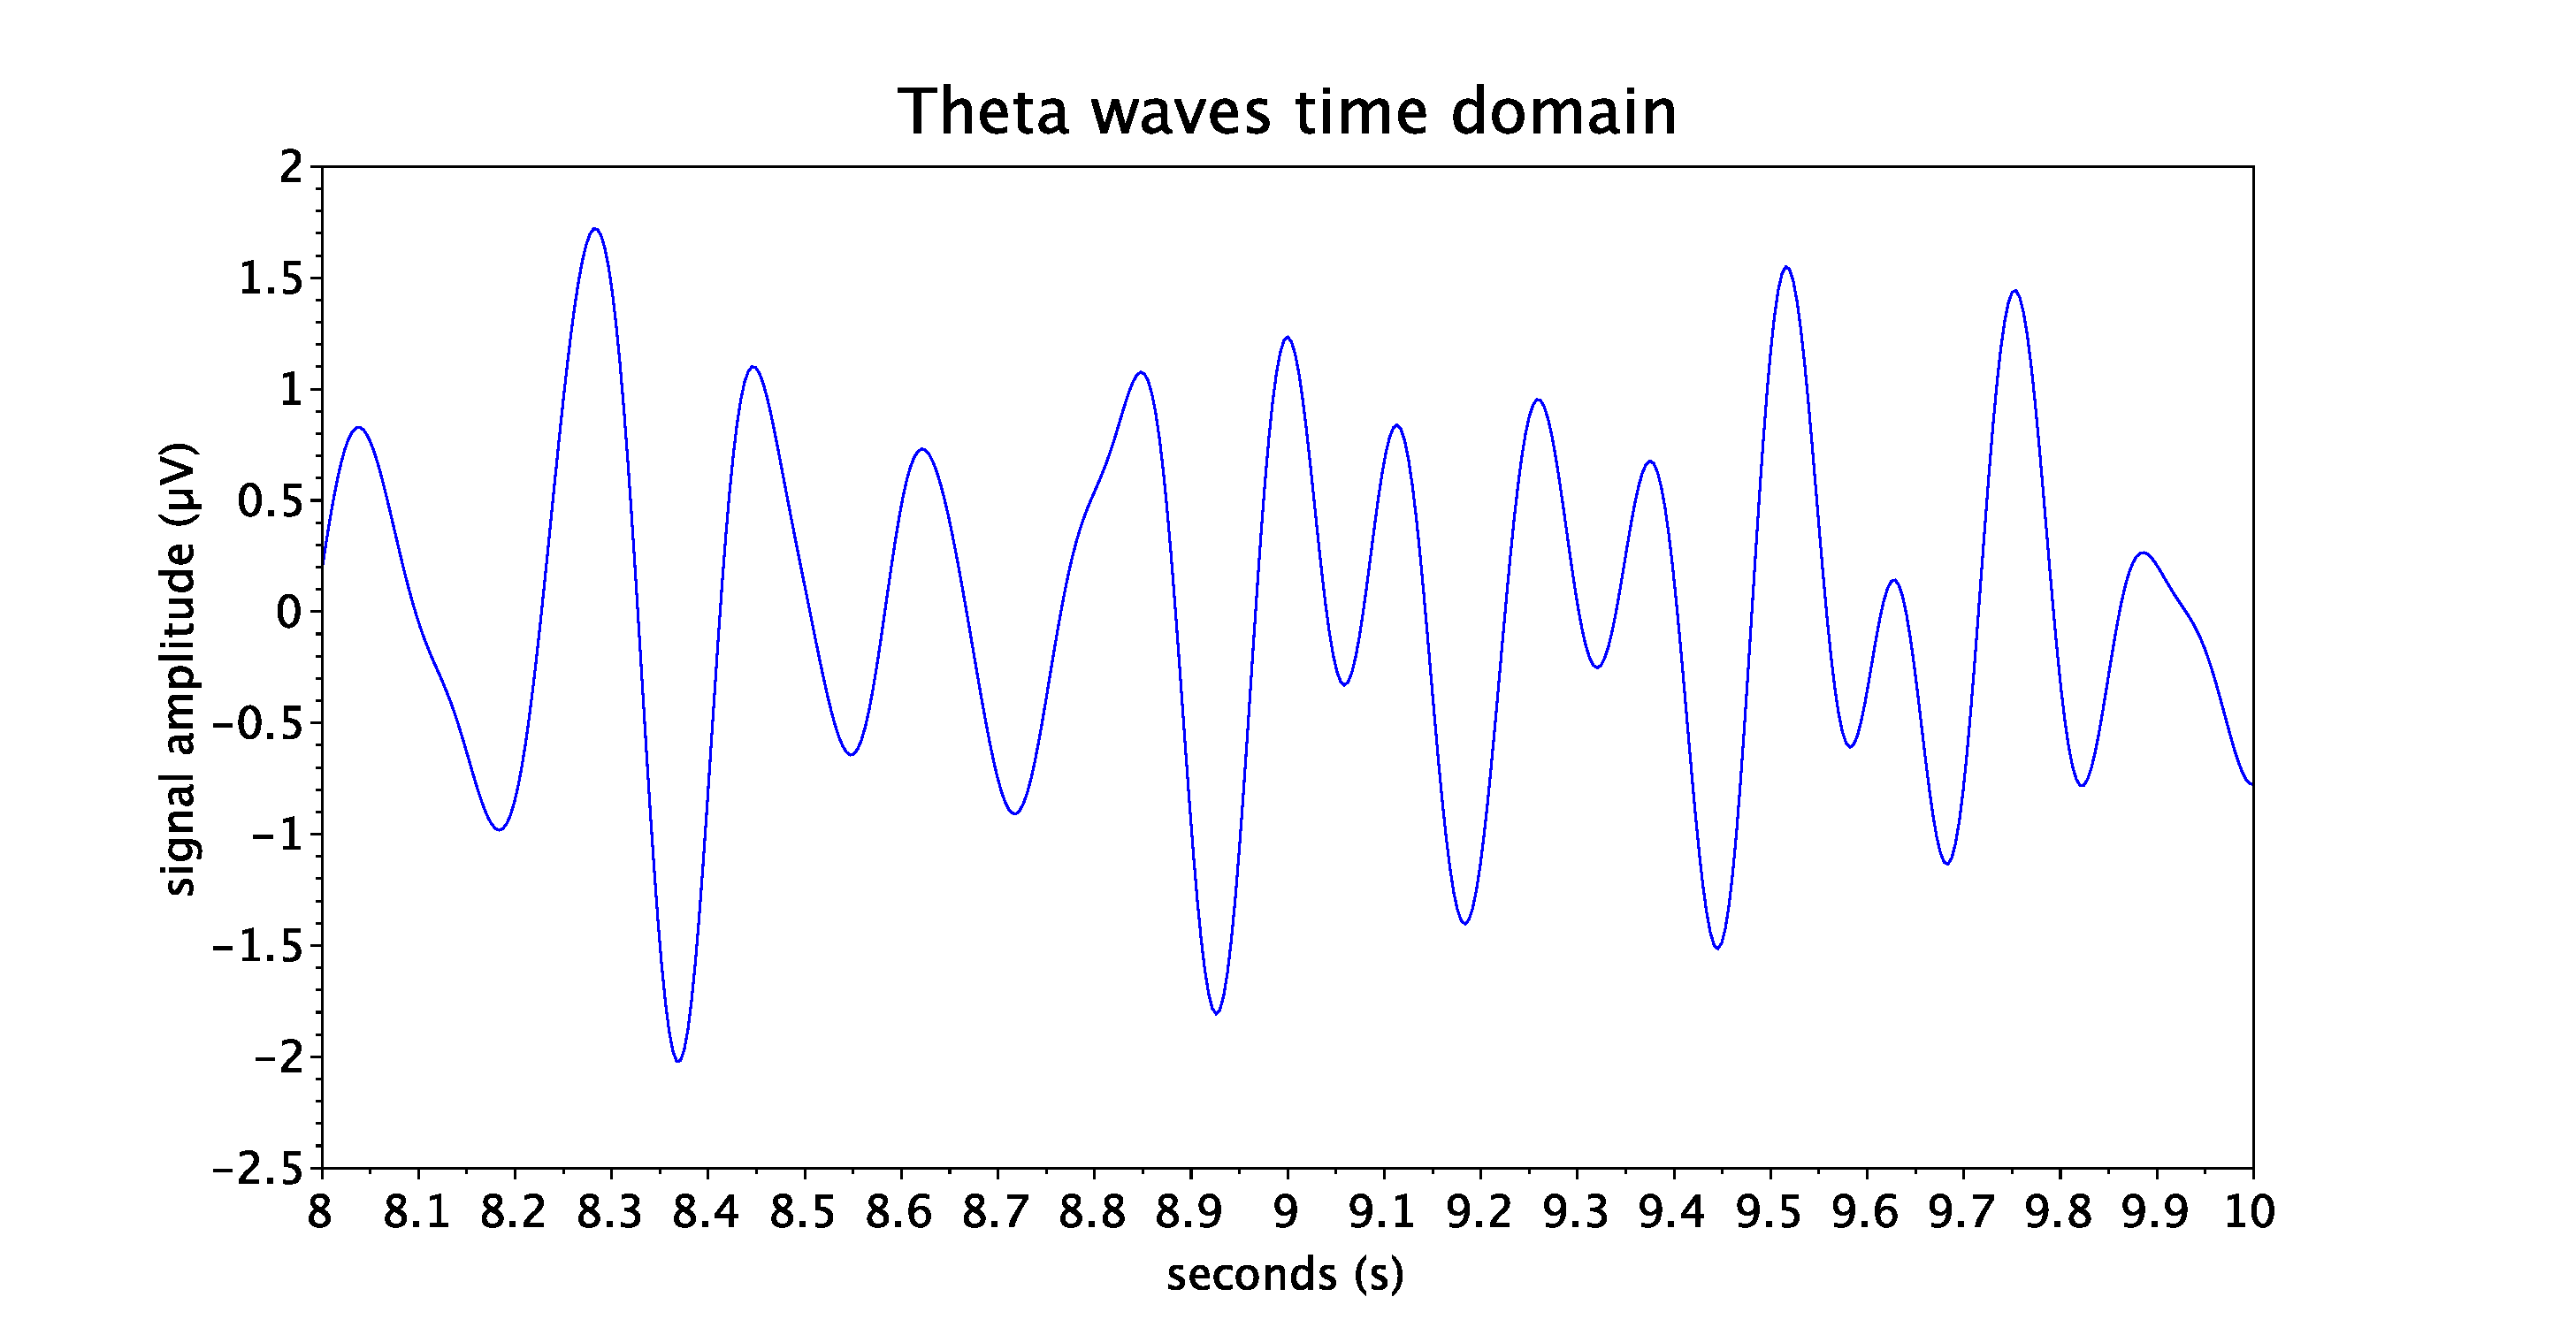
\includegraphics[width=\linewidth+3.2cm]{theta_time.pdf}
        \caption{Odczyt EEG z elektrody D19 w dziedzinie czasu}
    \end{figure}
    \begin{figure}[H]
        \hspace*{-1.5cm} 
        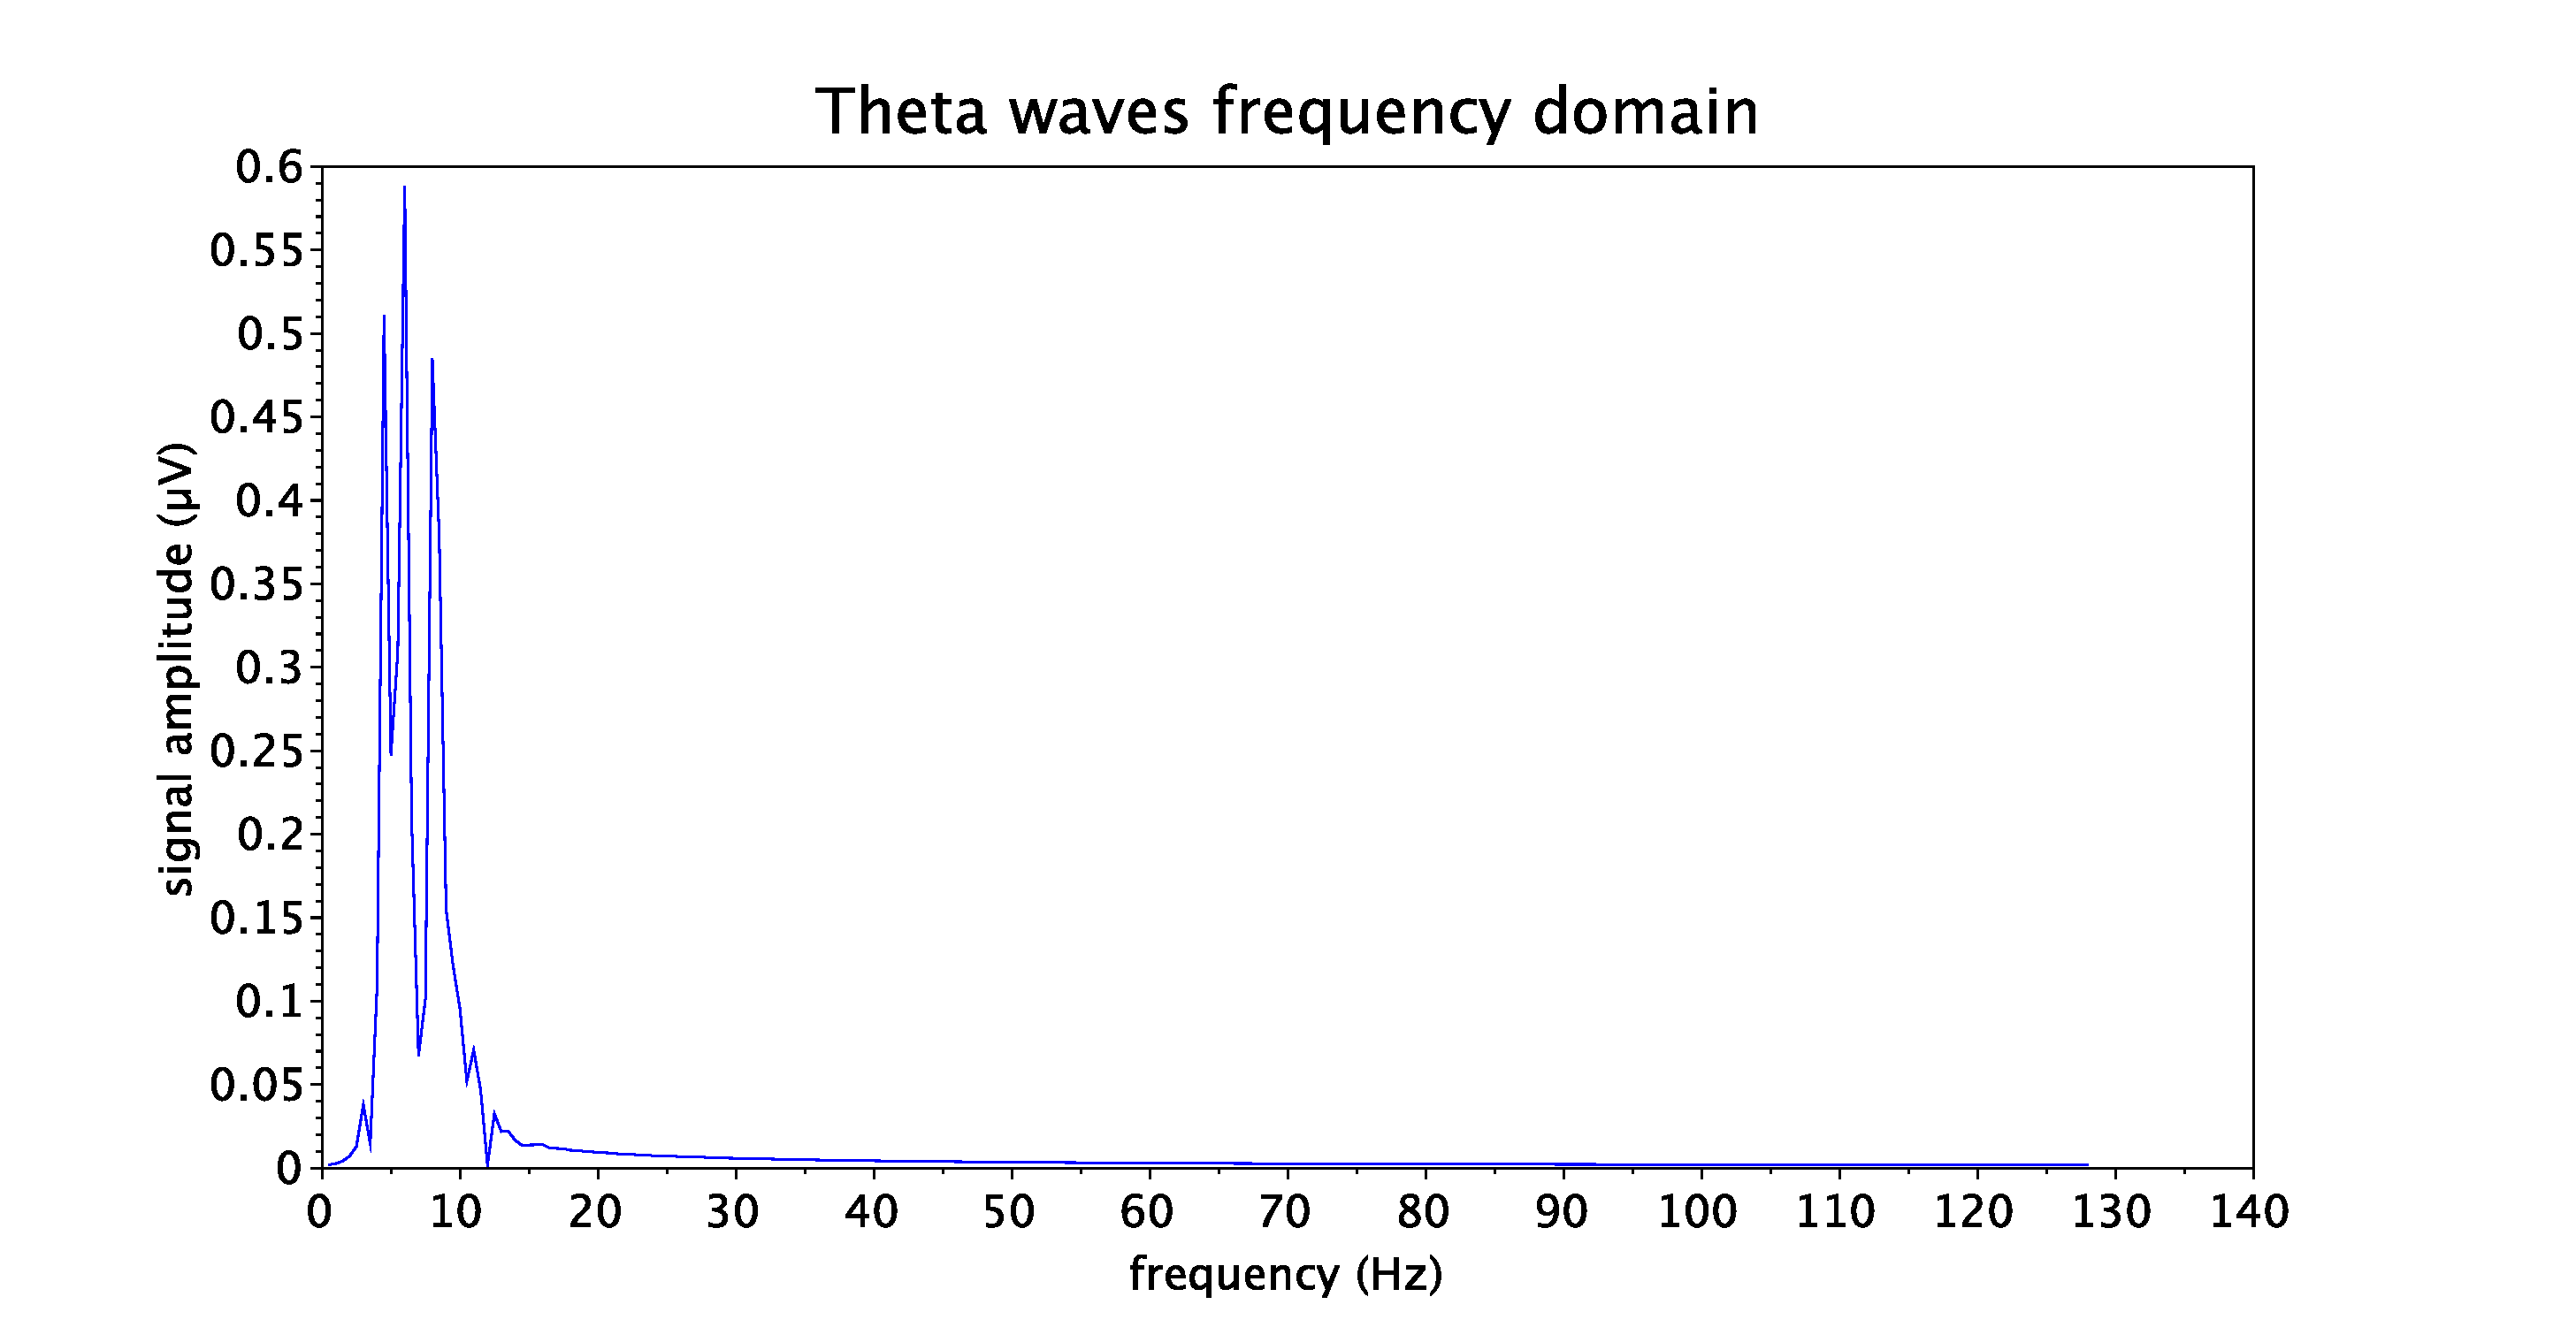
\includegraphics[width=\linewidth+3cm]{theta_freq.pdf}
        \caption{Odczyt EEG z elektrody D19 w dziedzinie częstotliwości}
    \end{figure}
% % %

\newpage
\section{Skrypt wraz z komentarzem}
\lstset{style=scilab}
\lstinputlisting[language=Scilab]{eeg_128.sce}
% % %

\newpage
\begin{thebibliography}{50}
    \bibitem{} Augustyniak P., \emph{Przetwarzanie sygnałów elektrodiagnostycznych}, AGH Uczelniane Wydawnictwa Naukowo-Dydaktyczne, 2001.
    \bibitem{} http://www.biosemi.com/pics/cap\_128\_layout\_medium.jpg
    \bibitem{} http://frontalcortex.com/images/eeg/1020labels.jpg        
    \bibitem{} http://zasoby.open.agh.edu.pl/~10swlabaj/fourier/skladowe.html
    \bibitem{} http://en.wikipedia.org/wiki/Electroencephalography
    \bibitem{} https ://brain.fuw.edu.pl/edu/EEG:Metody\_analizy\_sygna\%C5\%82\%C3\%B3w\_EEG\_-\_analiza\_w\_dziedzinie\_czasu
    \bibitem{} http://en.wikipedia.org/wiki/10-20\_system\_\%28EEG%29
\end{thebibliography}

% mdframed and alltt example %%%%%%%%%%%%%%%%%%%%%%%%%%%%
    %\begin{mdframed}
    %\begin{alltt}
    %signal\_mean   
    %    1.9177947  
    %\end{alltt}
    %\end{mdframed} 

\end{document}
